\documentclass[12pt,a4paper,twoside,openany]{report}

% Encoding et langues
\usepackage[french]{babel}

% Geometrie de la page
\usepackage[
  top=2.5cm,
  bottom=2.5cm,
  left=3cm,
  right=2.5cm,
  headheight=15pt,
  headsep=15pt,
  footskip=15pt
]{geometry}

% Packages essentiels
\usepackage{graphicx}
\usepackage{xcolor}
\usepackage{tikz}
\usetikzlibrary{positioning,shapes.geometric,arrows.meta,calc}
\usepackage{hyperref}
\usepackage{fancyhdr}
\usepackage{setspace}
\usepackage{amsmath}
\usepackage{amssymb}
\usepackage{array}
\usepackage{booktabs}
\usepackage{multirow}
\usepackage{caption}
\usepackage{subcaption}
\usepackage{float}
\usepackage{xurl}
\usepackage{enumitem}
\usepackage{parskip}
\usepackage{tabularx}
\usepackage{longtable}

% Espacement
\onehalfspacing

% En-tetes et pieds de page
\pagestyle{fancy}
\fancyhf{}
\fancyhead[LE,RO]{\small\textit{Conception d'un Agent de Reporting pour la Performance de Prestations}}
\fancyfoot[C]{\thepage}
\renewcommand{\headrulewidth}{0.5pt}
\renewcommand{\footrulewidth}{0pt}

% Hyperref
\hypersetup{
  colorlinks=true,
  linkcolor=darkblue,
  urlcolor=blue,
  citecolor=darkblue,
  bookmarks=true,
  bookmarksnumbered=true
}

\setcounter{tocdepth}{3}
\setcounter{secnumdepth}{3}

% Couleurs
\definecolor{darkblue}{RGB}{0,51,102}
\definecolor{lightblue}{RGB}{230,240,250}
\definecolor{padesce}{RGB}{26,82,118}

% Chemin des figures
\graphicspath{{figures/generated/}{figures/screenshots/}{figures/logos/}{figures/}}

% =====================================================
\begin{document}

\pagenumbering{roman}
\setcounter{page}{1}

% =====================================================
% PAGE DE COUVERTURE
% =====================================================

\begin{titlepage}
\begin{center}

\noindent
\begin{minipage}[t]{0.35\textwidth}
\raggedright
\begin{tikzpicture}
\node[inner sep=0pt] at (0,0) {\footnotesize\textsc{Ecole Superieure Francaise}};
\draw[fill=purple!80, rounded corners=3pt] (-1.2,-0.4) rectangle (1.2,-1.6);
\node[text=white, font=\bfseries\large] at (0,-1) {KEYCE};
\node[font=\tiny] at (0,-1.9) {\textit{Informatique \& Intelligence Artificielle}};
\node[font=\tiny] at (0,-2.2) {\textit{ISKIIA / ISKIMC}};
\end{tikzpicture}
\end{minipage}%
\hfill
\begin{minipage}[t]{0.55\textwidth}
\raggedleft
\textbf{REPUBLIQUE DU CAMEROUN}\\
\textit{Paix -- Travail -- Patrie}\\[0.3cm]
\textbf{MINISTERE DE L'ENSEIGNEMENT SUPERIEUR}
\end{minipage}

\vspace{2cm}

{\Large \textbf{KEYCE INFORMATIQUE ET INTELLIGENCE ARTIFICIELLE}}

\vspace{0.3cm}

\underline{Filiere : Intelligence Artificielle et Big Data}

\vspace{1.5cm}

{\LARGE \textbf{MEMOIRE DE FIN D'ETUDES}}

\vspace{0.5cm}

Presente en vue de l'obtention du diplome de

\vspace{0.3cm}

{\Large \textbf{\underline{Master 2 en Intelligence Artificielle et Big Data}}}

\vspace{1.5cm}

\fcolorbox{darkblue}{lightblue}{
\parbox{0.8\textwidth}{
\centering
\vspace{0.5cm}
{\large \textbf{\textcolor{darkblue}{Conception d'un agent de reporting pour la}}}

{\large \textbf{\textcolor{darkblue}{performance de prestations}}}
\vspace{0.5cm}
}
}

\vspace{1.5cm}

\textbf{Presente par :}

\vspace{0.3cm}

{\large EYOUM ATOCK JEAN-JACQUES BRAYAN}

\vspace{1cm}

\textbf{Sous la direction de :}

\vspace{0.5cm}

\begin{tabular}{p{0.45\textwidth}p{0.45\textwidth}}
\underline{\textbf{Encadreur Professionnel :}} & \underline{\textbf{Encadreur Academique :}} \\
M. EBONGUE Maxwell & M. FOMEKONG Evaris \\
 & Dr BILLONG IV Samuel Ismael \\
\end{tabular}

\vfill

\textbf{\textit{Annee Academique 2025--2026}}

\end{center}
\end{titlepage}

% =====================================================
% DEDICACE
% =====================================================

\chapter*{Dedicace}
\addcontentsline{toc}{chapter}{Dedicace}

\vspace{5cm}

\begin{center}
\textit{\Large A ma famille.}
\end{center}

\newpage

% =====================================================
% REMERCIEMENTS
% =====================================================

\chapter*{Remerciements}
\addcontentsline{toc}{chapter}{Remerciements}

Je tiens a exprimer ma sincere gratitude a mon encadreur academique, M. FOMEKONG Evaris, et a Dr BILLONG IV Samuel Ismael, pour leur accompagnement, leur disponibilite et la rigueur de leurs conseils tout au long de ce travail.

Mes remerciements s'adressent egalement a mon encadreur professionnel, M. EBONGUE Maxwell, pour son encadrement et pour l'acces aux donnees et au contexte professionnel ayant permis la realisation de ce memoire.

Je remercie l'ensemble du corps enseignant et administratif de KEYCE Informatique et Intelligence Artificielle pour la qualite de la formation dispensee.

Enfin, je remercie ma famille pour son soutien constant et ses encouragements tout au long de ce parcours.

\newpage

% =====================================================
% RESUME
% =====================================================

\chapter*{Resume}
\addcontentsline{toc}{chapter}{Resume}

{\setlength{\parskip}{0pt}
Ce memoire presente la conception d'un agent de reporting hybride -- regles metier explicites et intelligence artificielle generative -- pour evaluer la performance des prestataires de formation du PADESCE au Cameroun, pour le compte de NAUMUR. L'agent lit les donnees d'un prestataire (classeur Excel ou simple texte libre), les enrichit via une base de connaissances du contexte socio-geo-politique camerounais (reseau, electricite, securite, vocations economiques par region), pose des questions cibles si des informations manquent, puis calcule un score pondere sur huit criteres, aboutissant a une categorie -- Faible, Moyen ou Excellent -- accompagnee de recommandations d'investissement et d'un rapport PDF automatique avec commentaire genere par LLM (Llama/Groq).
Teste de bout en bout sur un cas reel (prestataire AMIFO-CIG, Sud-Ouest), l'agent produit un score de 75,9\,\% (Excellent) malgre une completude de donnees faible (25,8\,\%), compensee par un bon volume d'apprenants et une couverture geographique satisfaisante. La contribution principale est de montrer qu'un systeme interpretable et rapidement deployable offre au PADESCE un outil de pilotage plus utile qu'un modele d'apprentissage automatique, opaque et fragile sur un historique aussi limite.
}

\textbf{Mots-cles :} agent de reporting ; intelligence artificielle generative ; evaluation multicritere ; gouvernance des donnees ; Cameroun ; PADESCE.

\newpage

% =====================================================
% ABSTRACT
% =====================================================

\chapter*{Abstract}
\addcontentsline{toc}{chapter}{Abstract}

{\setlength{\parskip}{0pt}
This dissertation presents a hybrid reporting agent -- explicit business rules combined with generative artificial intelligence -- for evaluating the performance of PADESCE training providers in Cameroon, on behalf of NAUMUR. The agent reads provider data (an Excel workbook or plain free text), enriches it using a knowledge base of Cameroon's socio-geo-political context (network, electricity, security, regional economic vocations), asks targeted questions when information is missing, and computes a weighted score across eight criteria, yielding a category -- Weak, Average or Excellent -- together with investment recommendations and an automatic PDF report featuring LLM-generated commentary (Llama/Groq).
Tested end to end on a real case (provider AMIFO-CIG, South West region), the agent produced a score of 75.9\% (Excellent) despite low data completeness (25.8\%), offset by a solid learner volume and good geographic coverage. The main contribution is showing that an interpretable, quickly deployable system gives PADESCE a more useful steering tool than a machine-learning model, which would be opaque and fragile on such a limited historical dataset.
}

\textbf{Keywords:} reporting agent; generative artificial intelligence; multi-criteria evaluation; data governance; Cameroon; PADESCE.

\newpage

% =====================================================
% LISTES
% =====================================================

\listoftables
\newpage
\listoffigures
\newpage

% =====================================================
% SIGLES ET ABREVIATIONS
% =====================================================

\chapter*{Liste des sigles et abreviations}
\addcontentsline{toc}{chapter}{Liste des sigles et abreviations}

\begin{center}
\begin{tabular}{>{\bfseries}l p{11cm}}
\toprule
\textbf{Sigle} & \textbf{Signification} \\
\midrule
API & Interface de Programmation Applicative \\
HMAC & Code d'Authentification de Message par Hachage (\textit{Hash-based Message Authentication Code}) \\
IA & Intelligence Artificielle \\
LLM & Grand Modele de Langage (\textit{Large Language Model}) \\
MINESEC & Ministere des Enseignements Secondaires \\
NLU & Comprehension du Langage Naturel (\textit{Natural Language Understanding}) \\
PADESCE & Projet d'Appui au Developpement de l'Enseignement Secondaire et des Competences pour la Croissance et l'Emploi \\
PDF & Format de Document Portable (\textit{Portable Document Format}) \\
PII & Information Permettant d'Identifier une Personne \\
RAG & Generation Augmentee par Recuperation (\textit{Retrieval-Augmented Generation}) \\
SHA & Algorithme de Hachage Securise (\textit{Secure Hash Algorithm}) \\
UCP & Unite de Coordination du Projet \\
\bottomrule
\end{tabular}
\end{center}

\newpage

% =====================================================
% SOMMAIRE
% =====================================================

\tableofcontents

\newpage

% =====================================================
% INTRODUCTION GENERALE
% =====================================================

\pagenumbering{arabic}
\setcounter{page}{1}

\chapter*{Introduction generale}
\addcontentsline{toc}{chapter}{Introduction generale}

\section*{Contexte et justification}
\addcontentsline{toc}{section}{Contexte et justification}

Le pilotage d'un portefeuille de prestataires de formation ne se resume pas a la collecte de statistiques d'execution. Il exige de savoir, pour chaque prestataire et chaque zone d'intervention, si les conditions locales -- reseau, electricite, securite, vocations economiques -- ont ete prises en compte, et si les donnees remontees sont suffisamment fiables pour appuyer une decision d'investissement. Au Cameroun, ces conditions varient fortement d'une region a l'autre : un prestataire operant a Douala ne fait pas face aux memes contraintes qu'un prestataire operant a Kumba ou Bamenda, en zone anglophone affectee par une crise securitaire prolongee.

Le PADESCE vise notamment l'amelioration de l'acces equitable a un enseignement secondaire de qualite et le developpement de competences adaptees au marche du travail, avec une attention particuliere portee aux filles (WORLD BANK, 2020). Son cadre de resultats associe plusieurs niveaux de mesure et prevoit des mecanismes de verification independante. Les equipes de suivi de NAUMUR, chargees d'appeler les beneficiaires et de compiler les donnees des prestataires, disposent de fichiers Excel heterogenes -- listes d'apprenants, calendriers de seances -- dont la structure et la qualite varient d'un prestataire a l'autre, et n'ont pas toujours le temps ni l'expertise pour resituer chaque prestataire dans son contexte regional avant de rendre un avis.

Un systeme d'aide au reporting peut combler cet ecart, a condition de rester interpretable, rapide a deployer et gouvernable : il doit pouvoir justifier chacune de ses evaluations, fonctionner avec les fichiers reellement produits sur le terrain, et ne pas exiger un historique de donnees dont le PADESCE ne dispose pas encore en quantite suffisante pour entrainer un modele statistique robuste.

\section*{Problematique}
\addcontentsline{toc}{section}{Problematique}

Les donnees disponibles pour chaque prestataire sont partielles et heterogenes : un classeur Excel de liste d'apprenants et de calendrier, parfois complete d'informations orales transmises par telephone ou par courriel sous forme de texte libre. Aucune base de donnees historique suffisamment large et stable ne permet, a ce stade, d'entrainer et de valider statistiquement un modele predictif de la performance d'un prestataire. La question devient alors : comment evaluer, de maniere reproductible, justifiable et utilisable immediatement, la performance d'un prestataire a partir de donnees incompletes et d'un contexte local qu'il faut reconstituer manuellement a chaque fois ?

La difficulte centrale ne consiste donc pas a ajuster les hyperparametres d'un algorithme d'apprentissage, mais a concevoir un systeme qui (i) nettoie et interprete des donnees Excel non standardisees, (ii) injecte automatiquement une connaissance contextuelle du Cameroun que l'evaluateur humain devrait sinon reconstituer a chaque dossier, (iii) pose les bonnes questions quand l'information manque, et (iv) produit un jugement explicable et actionnable pour le PADESCE.

\section*{Questions de recherche}
\addcontentsline{toc}{section}{Questions de recherche}

La question principale est formulee ainsi :

\begin{quote}
\textit{Comment concevoir un agent de reporting hybride, combinant regles metier explicites et intelligence artificielle generative, capable d'evaluer la performance d'un prestataire du PADESCE a partir de donnees heterogenes et d'un contexte camerounais codifie, tout en restant interpretable et gouvernable ?}
\end{quote}

Elle se decline en trois sous-questions :

\begin{description}[leftmargin=1cm]
\item[QR1.] Quelles regles de nettoyage et d'analyse permettent d'extraire une information fiable de classeurs Excel de prestataires non standardises ?
\item[QR2.] Comment structurer une base de connaissances socio-geo-demographique et politique du Cameroun de maniere a enrichir automatiquement l'evaluation sans que l'utilisateur ait a la re-expliquer a chaque fois ?
\item[QR3.] Quelle architecture de scoring multicritere, ponderee et justifiee, permet de produire une categorie de performance (Faible, Moyen, Excellent) exploitable pour orienter les decisions d'investissement du PADESCE ?
\end{description}

\section*{Hypotheses}
\addcontentsline{toc}{section}{Hypotheses}

Les hypotheses de travail suivantes structurent la conception et sont discutees au regard du cas reel traite :

\begin{description}[leftmargin=1cm]
\item[H1.] Un systeme de scoring a regles explicites et ponderees, complete par une couche d'IA generative pour la narration, offre un meilleur compromis interpretabilite/utilite operationnelle qu'un modele d'apprentissage automatique entraine sur un historique de prestataires trop restreint pour generaliser.
\item[H2.] L'enrichissement automatique par une base de connaissances regionale codee en dur ameliore la pertinence de l'evaluation par rapport a une evaluation qui ignorerait le contexte local (reseau, electricite, securite, vocations economiques).
\item[H3.] Le nettoyage et la normalisation des classeurs Excel heterogenes constituent le facteur limitant principal de la qualite du score, davantage que la sophistication de l'algorithme de ponderation.
\end{description}

\section*{Objectifs}
\addcontentsline{toc}{section}{Objectifs}

L'objectif general est de concevoir, implementer et tester un agent de reporting hybride pour l'evaluation de la performance des prestataires du PADESCE et d'en demontrer l'utilite sur un cas reel.

Les objectifs specifiques consistent a :

\begin{enumerate}
\item concevoir un module d'ingestion et de nettoyage capable de traiter des classeurs Excel de prestataires non standardises ;
\item construire et documenter une base de connaissances socio-geo-demographique et politique des dix regions du Cameroun ;
\item concevoir un systeme de scoring multicritere pondere, avec justification textuelle par critere ;
\item integrer une couche d'intelligence artificielle generative pour la production d'un commentaire narratif, avec repli automatique en l'absence d'acces a l'API ;
\item generer un rapport PDF brande NAUMUR et le tester sur un cas reel de prestataire (AMIFO-CIG) ;
\item proposer un cadre de protection des donnees personnelles des apprenants et de gouvernance de l'usage du score.
\end{enumerate}

\section*{Interet scientifique et pratique}
\addcontentsline{toc}{section}{Interet scientifique et pratique}

Sur le plan scientifique, le memoire documente la conception d'un agent hybride regles + IA generative pour une tache d'evaluation multicritere en contexte de donnees rares, et explicite le raisonnement ayant conduit a ecarter un modele d'apprentissage automatique purement statistique au profit d'un systeme interpretable -- un choix de conception rarement justifie de maniere aussi explicite dans la litterature appliquee.

Sur le plan pratique, le travail fournit au PADESCE et a NAUMUR un outil operationnel : un agent capable de transformer un classeur Excel brut ou une description en langage naturel en un rapport PDF exploitable en quelques secondes, incluant alertes, recommandations d'investissement et commentaire narratif, sans attendre la constitution d'un historique de donnees suffisant pour un modele statistique.

\section*{Organisation du memoire}
\addcontentsline{toc}{section}{Organisation du memoire}

Le premier chapitre precise les concepts, les cadres theoriques et les travaux anterieurs relatifs aux agents de reporting, a l'IA generative et a l'evaluation multicritere. Le deuxieme decrit la methodologie de conception de l'agent, de la base de connaissances et du systeme de scoring. Le troisieme presente le contexte technique, l'implementation et les resultats obtenus sur le cas reel AMIFO-CIG. Le quatrieme discute les limites et propose des pistes d'intervention. Une conclusion generale recapitule les contributions et les prolongements necessaires.

\newpage

% =====================================================
% CHAPITRE 1
% =====================================================

\chapter{Cadre conceptuel, theorique et etat de l'art}

\section{Clarification des concepts metier}

\subsection{Performance d'une prestation de formation}

Le terme performance est polysemique. Dans le present travail, il designe le degre auquel un prestataire de formation a mobilise, dans des conditions adaptees a son contexte local, des ressources suffisantes et diversifiees pour atteindre des beneficiaires dans de bonnes conditions. Cette definition operationnelle se distingue volontairement d'une mesure de satisfaction declarative ou d'un indicateur d'insertion professionnelle : elle porte sur ce qui peut etre observe et verifie a partir des donnees administratives et logistiques disponibles au moment du reporting -- nombre d'apprenants, diversite des formations, couverture geographique, planification -- combinees a une appreciation du contexte dans lequel le prestataire opere.

\subsection{Agent de reporting}

Un agent de reporting, tel qu'entendu ici, est un systeme logiciel qui recoit des donnees brutes, les enrichit d'une connaissance contextuelle, applique des regles d'evaluation explicites, sollicite au besoin un complement d'information aupres de l'utilisateur, puis produit un document de synthese destine a la decision. Il se distingue d'un simple tableau de bord par sa capacite a raisonner sur des donnees incompletes et heterogenes, et d'un modele d'apprentissage automatique par le caractere explicite et modifiable de ses regles de decision.

\subsection{Intelligence artificielle generative et grands modeles de langage}

Un grand modele de langage (LLM) est un reseau de neurones entraine sur de vastes corpus textuels, capable de produire du texte coherent en reponse a une instruction (\textit{prompt}). Dans l'agent concu ici, un LLM (Llama, servi via l'API Groq) n'intervient pas dans le calcul du score -- qui reste entierement determine par des regles ponderees -- mais dans la redaction du commentaire narratif accompagnant le rapport, a partir d'un prompt structure contenant les donnees et le score deja calcules. Cette separation entre calcul deterministe et generation narrative est un choix de conception central, discutee a la section~\ref{sec:positionnement}.

\subsection{Evaluation multicritere}

L'evaluation multicritere consiste a agreger plusieurs dimensions de jugement, chacune ponderee selon son importance relative, en un score unique interpretable. Elle est couramment utilisee dans l'evaluation de projets de developpement, ou une decision (financer, suspendre, accompagner) doit s'appuyer sur plusieurs criteres simultanement -- pertinence, efficacite, efficience, impact, durabilite selon les criteres du Comite d'aide au developpement de l'OCDE (OECD, 2019, 2021). Le systeme concu dans ce memoire applique ce principe a l'echelle d'un prestataire individuel, avec huit criteres ponderes (section~\ref{sec:criteres}).

\section{Clarification des concepts techniques}

\subsection{Systeme a regles versus apprentissage statistique}

Un systeme a regles explicites encode directement la connaissance metier sous forme de conditions et de ponderations verifiables par un humain. Un modele d'apprentissage supervise, a l'inverse, infere une fonction de decision a partir d'exemples historiques, au prix d'une perte partielle d'interpretabilite et d'une dependance a la taille et a la representativite de l'echantillon d'entrainement. Lorsque l'echantillon disponible est petit et le risque de surapprentissage eleve, la litterature invite a la prudence quant a la generalisation d'un modele statistique complexe (CAWLEY \& TALBOT, 2010 ; VARMA \& SIMON, 2006). C'est precisement le cas des donnees de prestataires du PADESCE au moment de la conception de cet agent : le nombre de dossiers de prestataires disponibles est trop faible pour entrainer et valider statistiquement un modele predictif fiable, ce qui motive le choix d'un systeme a regles, detaille a la section~\ref{sec:positionnement}.

\subsection{Enrichissement contextuel et generation augmentee}

L'enrichissement contextuel consiste a completer une donnee brute par une connaissance externe structuree avant de la traiter. Dans les systemes conversationnels modernes, cette logique est formalisee par la generation augmentee par recuperation (\textit{Retrieval-Augmented Generation}, RAG), qui consiste a injecter dans le contexte d'un LLM des informations pertinentes recuperees d'une base documentaire au moment de la requete. L'agent concu ici applique une version simplifiee et deterministe de ce principe : plutot qu'une recherche semantique dans un corpus ouvert, il effectue une correspondance directe (ville ou region citee \(\rightarrow\) fiche contextuelle) dans une base de connaissances codee en dur (module \texttt{cameroon\_context.py}), ce qui garantit une reponse stable, verifiable et sans risque d'hallucination sur les faits geographiques mobilises.

\subsection{Qualite et gouvernance des donnees}

La qualite des donnees ne se reduit pas a l'absence de valeurs manquantes. Elle comprend la tracabilite de la source, la coherence des definitions, la plausibilite des valeurs et la stabilite des identifiants (villes, prestataires). Dans un systeme d'information, la qualite de l'information conditionne l'utilite du dispositif pour l'utilisateur et l'organisation (DELONE \& MCLEAN, 2003). La gouvernance proposee dans ce memoire repose sur quatre principes : premierement, les identifiants directs des apprenants ne quittent jamais le fichier source operationnel sous forme lisible dans les extractions d'etude ; deuxiemement, le score ne peut appuyer une decision defavorable sans revue humaine documentee ; troisiemement, la base de connaissances Cameroun est versionnee et datee ; quatriemement, chaque rapport genere conserve la trace du fichier source, de l'horodatage et des reponses complementaires fournies. Ces principes rejoignent les fonctions de gouvernance, de mesure et de gestion du risque formulees dans le cadre du NIST pour les systemes d'intelligence artificielle (TABASSI, 2023).

\section{Cadres theoriques mobilises}

Le travail articule trois cadres complementaires. Le premier est le cadre d'evaluation de la formation de Kirkpatrick, qui distingue la reaction, l'apprentissage, le comportement et les resultats (KIRKPATRICK, 1996) ; il rappelle que les donnees disponibles au moment du reporting (volume, diversite, planification) renseignent surtout la mise en \oe uvre logistique d'une formation, et non son impact ulterieur -- ce que l'agent ne pretend pas mesurer. La figure~\ref{fig:kirkpatrick} illustre cette hierarchie.

\begin{figure}[H]
\centering
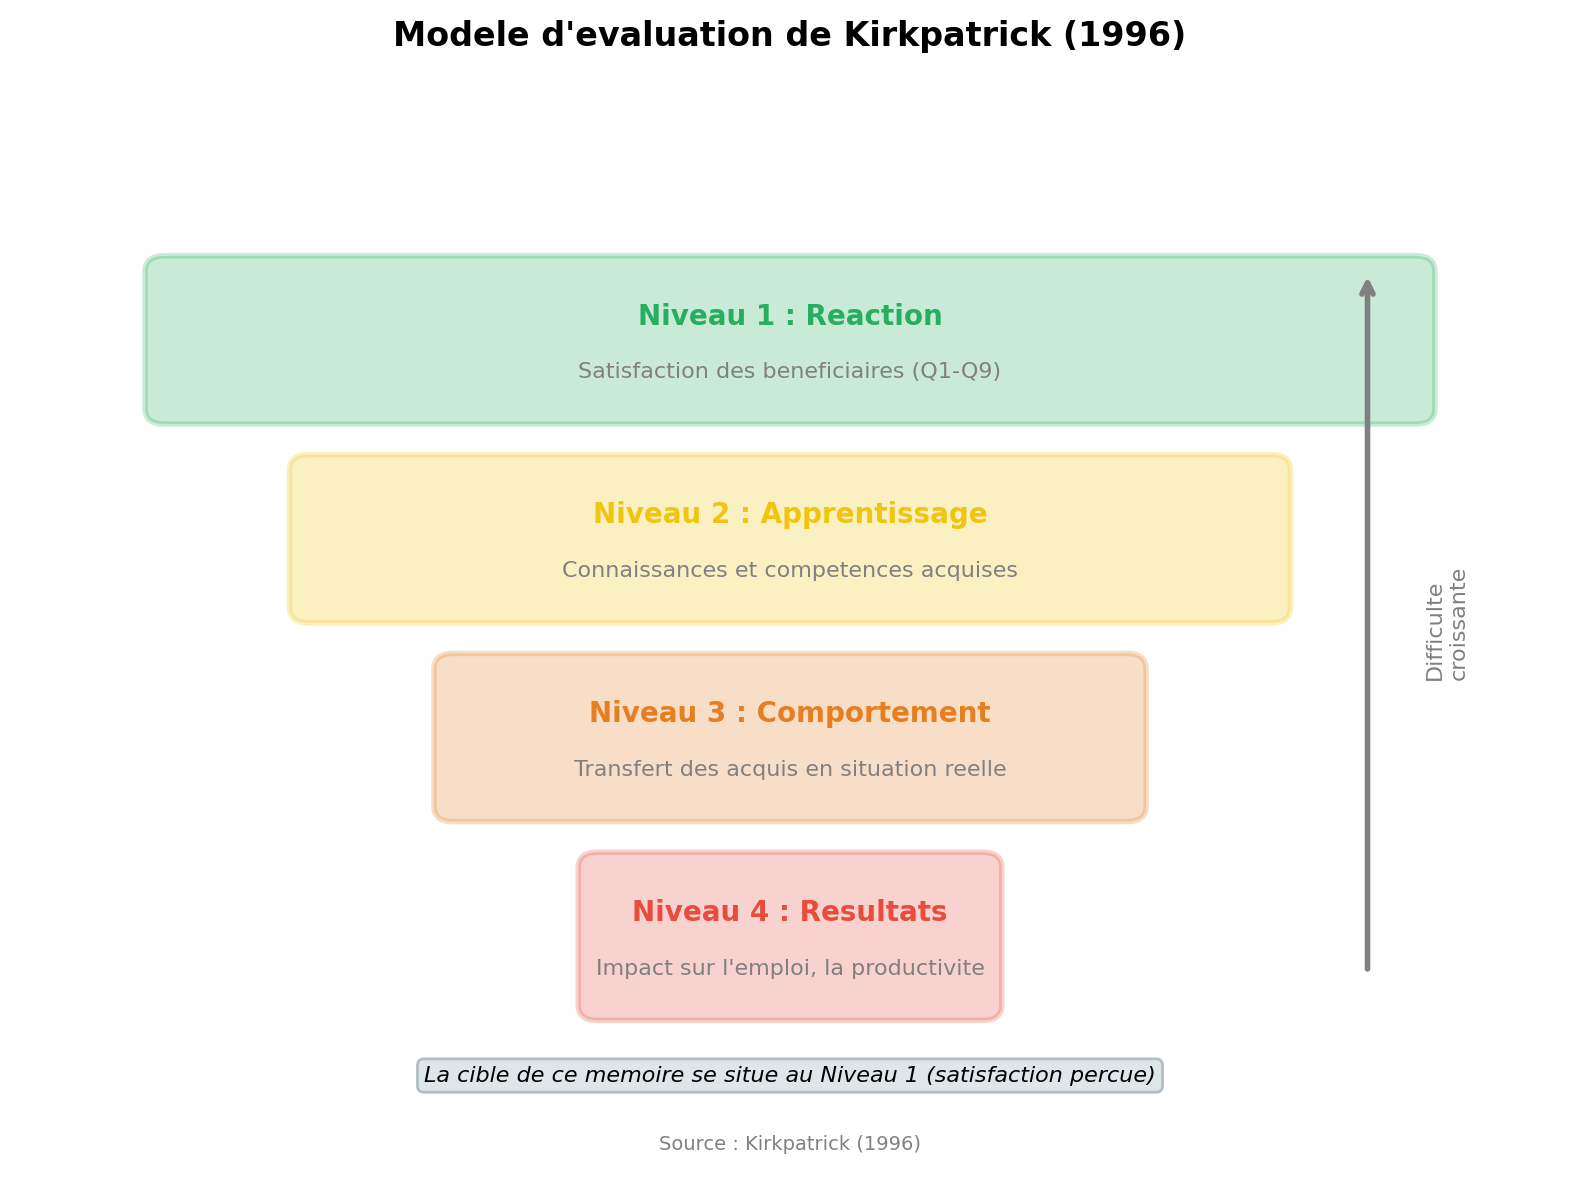
\includegraphics[width=0.75\textwidth]{kirkpatrick_niveaux.png}
\caption{Les quatre niveaux d'evaluation de Kirkpatrick}
\label{fig:kirkpatrick}
\textit{Source : Adapte de Kirkpatrick (1996).}
\end{figure}

Le deuxieme cadre est celui de l'evaluation multicritere ponderee, tel que promu par les criteres d'evaluation de l'OCDE pour les projets de developpement (OECD, 2019, 2021) : la performance globale resulte de l'agregation de dimensions partiellement independantes, chacune justifiee separement plutot que fondue dans un score opaque. Le troisieme est le principe de transparence algorithmique -- documenter les donnees utilisees (GEBRU et al., 2021) et le fonctionnement d'un systeme de decision (MITCHELL et al., 2019) -- qui justifie que chaque critere de l'agent produise une justification textuelle lisible, plutot qu'un score seul.

\section{Etat de l'art}

\subsection{Prediction et scoring dans les dispositifs de formation}

Les travaux de prediction educative se concentrent frequemment sur le risque d'abandon ou la reussite individuelle a partir d'historiques de traces d'apprentissage. Zeng et ses coauteurs etudient l'abandon dans une formation aux soins a domicile (ZENG et al., 2017). Gitinabard et ses coauteurs comparent plusieurs modeles pour identifier precocement les apprenants en difficulte dans des cours en ligne (GITINABARD et al., 2018). Al-Shabandar et ses coauteurs analysent des traces d'apprentissage en ligne a l'aide de plusieurs algorithmes (AL-SHABANDAR et al., 2019). Durdevic Babic mobilise des methodes de fouille de donnees pour predire la satisfaction a partir de journaux d'une plateforme d'apprentissage (DURDEVIC BABIC, 2015). Alshahrani propose un cadre d'apprentissage automatique optimise pour predire la retention dans des formations professionnelles (ALSHAHRANI, 2025).

Ces travaux partagent deux caracteristiques qui les rendent difficilement transposables au contexte du present memoire : ils supposent un historique de donnees suffisamment volumineux pour entrainer et valider statistiquement un modele, et leur unite d'analyse est generalement l'apprenant individuel plutot que le prestataire dans son contexte territorial. Le PADESCE, au moment de la conception de l'agent, ne dispose pas d'un tel historique consolide par prestataire ; et la decision a soutenir (financer, suspendre, accompagner un prestataire) porte sur le prestataire et son contexte local, non sur un apprenant isole.

\subsection{Agents et systemes d'aide a la decision augmentes par IA generative}

L'essor des grands modeles de langage a fait emerger des architectures dites « agentiques », dans lesquelles un LLM est combine a des outils externes (calcul, recherche documentaire, bases de connaissances) pour produire des reponses ancrees dans des donnees verifiables plutot que dans la seule memoire parametrique du modele. La generation augmentee par recuperation illustre ce principe pour la reduction des erreurs factuelles. L'agent concu dans ce memoire s'inscrit dans cette famille, mais avec une repartition des roles stricte : le LLM ne decide jamais du score -- qui reste calcule par des regles deterministes et auditable -- et n'intervient que pour la mise en recit du resultat deja etabli, ce qui limite le risque d'hallucination sur les chiffres rapportes dans le PDF final.

\subsection{Comparaison structuree des approches}

Le tableau~\ref{tab:comparaison_lit} compare les approches recensees selon six criteres : C1, fonctionnement avec un historique de donnees restreint ; C2, unite d'analyse au niveau du prestataire (et non de l'apprenant) ; C3, prise en compte explicite du contexte territorial ; C4, interpretabilite native du score ; C5, capacite a fonctionner sur donnees d'entree heterogenes (Excel non standardise ou texte libre) ; C6, production directe d'un livrable de decision (rapport).

\begin{table}[H]
\centering
\caption{Comparaison des approches de prediction/evaluation dans les dispositifs de formation}
\label{tab:comparaison_lit}
\begin{tabular}{l cccccc}
\toprule
\textbf{Approche} & \textbf{C1} & \textbf{C2} & \textbf{C3} & \textbf{C4} & \textbf{C5} & \textbf{C6} \\
\midrule
Zeng et al. (2017) & -- & -- & -- & -- & -- & -- \\
Gitinabard et al. (2018) & -- & -- & -- & -- & -- & -- \\
Al-Shabandar et al. (2019) & -- & -- & -- & -- & -- & -- \\
Durdevic Babic (2015) & -- & -- & -- & -- & -- & -- \\
Alshahrani et al. (2025) & -- & -- & -- & -- & -- & -- \\
\midrule
\textbf{Agent de reporting propose} & $\checkmark$ & $\checkmark$ & $\checkmark$ & $\checkmark$ & $\checkmark$ & $\checkmark$ \\
\bottomrule
\end{tabular}
\end{table}

\section{Positionnement de la recherche}
\label{sec:positionnement}

Le memoire adopte une posture de conception d'un systeme interpretable et rapidement deployable, deliberement ecartee d'un modele d'apprentissage automatique entraine sur un historique de prestataires. Ce choix n'est pas une facilite : il est justifie par trois arguments.

Premierement, l'echantillon de dossiers de prestataires disponibles au moment de la conception est trop restreint pour esperer une generalisation statistique fiable ; sur un tel echantillon, un modele complexe (foret aleatoire, boosting) tend a memoriser des particularites de l'echantillon d'entrainement plutot qu'a capter une relation generalisable (BREIMAN, 2001 ; CAWLEY \& TALBOT, 2010). Deuxiemement, un modele boite noire ne permettrait pas de justifier a un gestionnaire PADESCE pourquoi tel prestataire recoit tel score -- alors que la traçabilite critere par critere est une exigence operationnelle explicite du commanditaire. Des methodes d'explicabilite post-hoc existent (LIME : RIBEIRO et al., 2016 ; SHAP : LUNDBERG \& LEE, 2017), mais elles approxi\-ment un modele deja opaque plutot que d'offrir une transparence native. Troisiemement, le systeme doit pouvoir evoluer rapidement -- ajouter un critere, corriger une ponderation, mettre a jour une fiche regionale -- sans cycle de reentrainement, ce qu'un systeme a regles permet directement.

L'agent propose combine donc trois composantes : un moteur de regles pour le score (transparent, ponderable, modifiable sans reentrainement), une base de connaissances Cameroun codee en dur (garantissant l'absence d'hallucination sur les faits geographiques), et un LLM cantonne a la generation narrative (pour la lisibilite du rapport, avec repli automatique par gabarit si l'API est indisponible). Ce n'est ni un modele d'apprentissage automatique pur, ni un chatbot generatif pur, mais une architecture hybride ou chaque composante est utilisee pour ce qu'elle fait le mieux.

\textbf{Synthese du chapitre.} Ce chapitre a defini la performance d'une prestation dans son acception operationnelle, distingue l'agent de reporting d'un tableau de bord ou d'un modele statistique, et situe le role du LLM comme generateur de narration plutot que decideur. Il a montre que la litterature de prediction educative suppose generalement un historique de donnees dont le PADESCE ne dispose pas encore, ce qui justifie le choix d'une architecture hybride regles + IA generative. Le chapitre suivant formalise la methodologie de conception de cette architecture.

\newpage

% =====================================================
% CHAPITRE 2
% =====================================================

\chapter{Methodologie de recherche}

\section{Nature et dessin de l'etude}

La recherche adopte un dessin de conception et d'ingenierie logicielle (\textit{design science}), evalue par un cas d'usage reel plutot que par une validation statistique sur echantillon. L'objectif n'est pas d'estimer la generalisation d'un modele predictif, mais de concevoir un artefact -- l'agent de reporting -- puis de verifier qu'il produit, sur des donnees reelles, une evaluation coherente, justifiee et actionnable.

La figure~\ref{fig:architecture} presente l'architecture generale de l'agent, organisee en six modules Python independants et testables separement.

\begin{figure}[H]
\centering
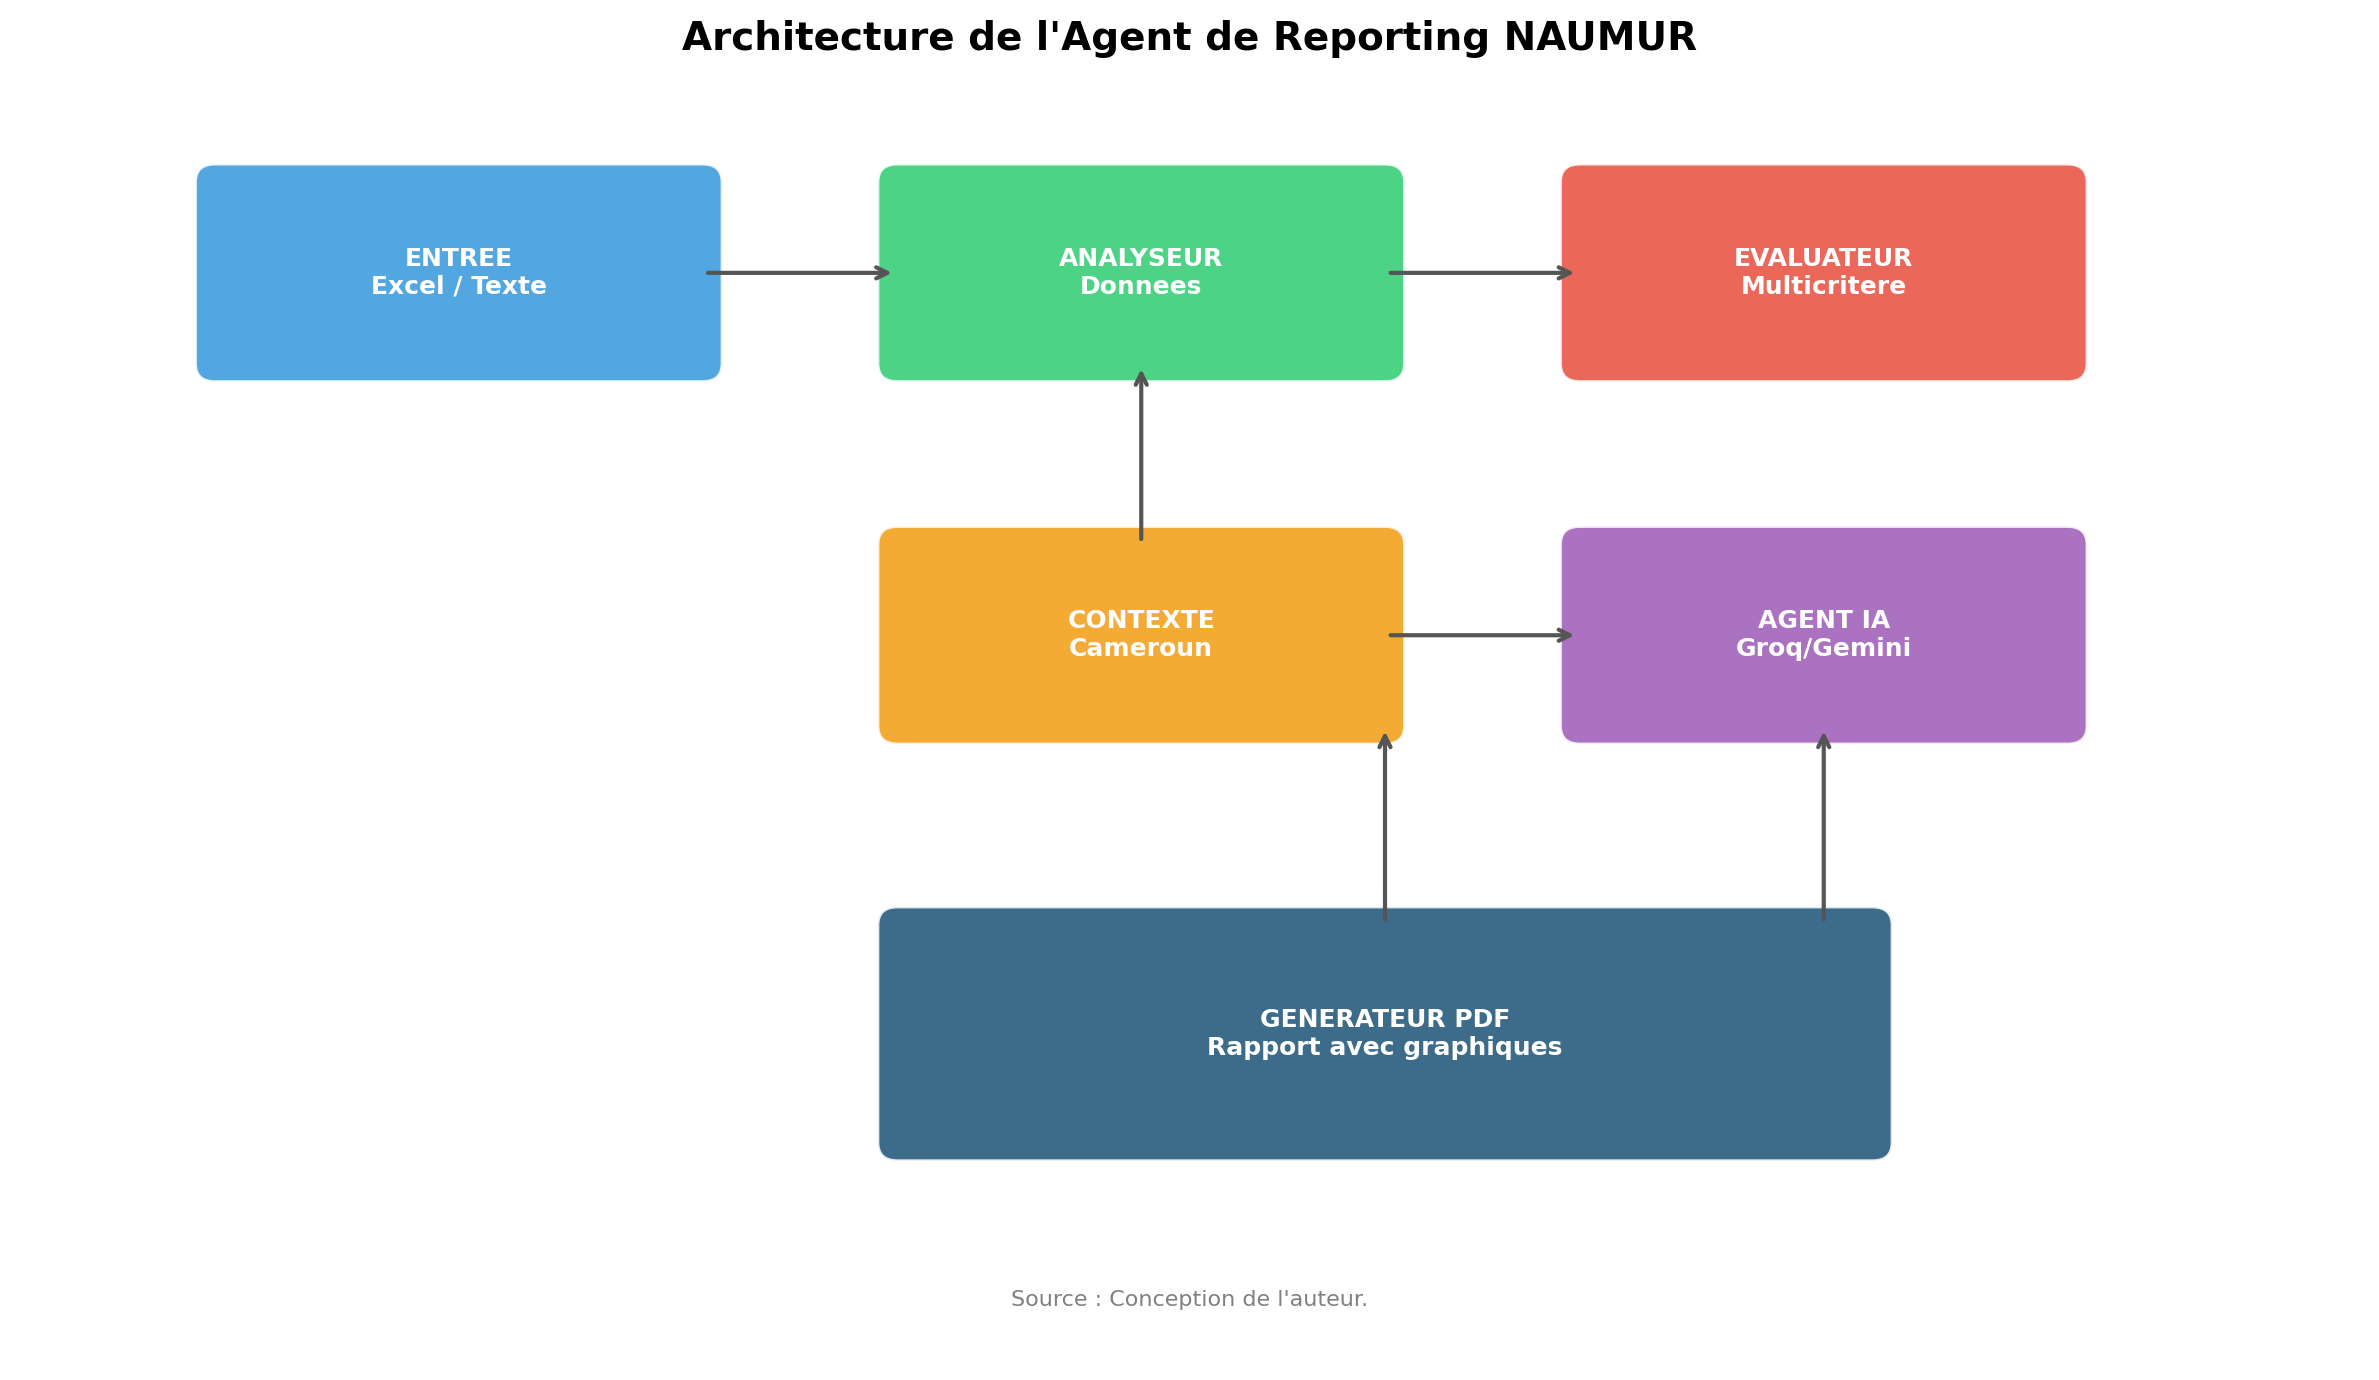
\includegraphics[width=0.95\textwidth]{architecture_agent.png}
\caption{Architecture modulaire de l'agent de reporting NAUMUR}
\label{fig:architecture}
\textit{Source : Elaboration de l'auteur.}
\end{figure}

\section{Conception du module d'ingestion et de nettoyage des donnees}

Le module \texttt{data\_analyzer.py} accepte un classeur Excel dont la structure n'est pas standardisee entre prestataires : noms de colonnes variables (« Nom », « Nom et prenom »), feuilles multiples (liste d'apprenants, calendrier de seances), et graphies incoherentes des noms de villes. La strategie de nettoyage retenue repose sur trois mecanismes.

Premierement, une detection de colonnes par mots-cles plutot que par position ou nom exact : chaque champ recherche (nom, genre, ville, formation, date) est identifie par une liste de synonymes possibles (par exemple \texttt{["ville", "city", "residence"]}), ce qui tolere les variations de nommage d'un fichier a l'autre. Deuxiemement, la suppression des lignes et colonnes entierement vides et des colonnes generees automatiquement par Excel (\texttt{Unnamed: *}). Troisiemement, un calcul de completude par colonne (proportion de cellules non vides), moyenne ensuite pour obtenir un score de completude global du fichier, utilise directement comme premier critere d'evaluation.

Une limite assumee de cette version est l'absence de deduplication automatique des graphies de villes : dans le cas reel traite (chapitre 3), la ville de Kumba apparait a la fois sous les graphies « KUMBA » et « Kumba », ce qui gonfle artificiellement le nombre de lieux distincts detectes. Ce point est repris dans la discussion des limites (chapitre 4) comme priorite d'amelioration du pretraitement.

\section{Construction de la base de connaissances Cameroun}

La base de connaissances (\texttt{cameroon\_context.py}) a ete construite en documentant, pour chacune des dix regions du Cameroun, sept dimensions : chef-lieu, population estimee, fiabilite du reseau mobile, fiabilite de l'electricite, qualite d'acces routier, defis specifiques (securitaires, climatiques, logistiques) et un score de difficulte synthetique compris entre 0 et 1. Chaque region est en outre associee a une liste de vocations economiques locales et de formations recommandees, utilisees pour evaluer la pertinence sectorielle des formations dispensees par un prestataire.

Une deuxieme table associe seize villes frequemment citees dans les dossiers de prestataires (Douala, Yaounde, Bamenda, Kumba, Foumban, etc.) a leur region, leur departement et des particularites locales -- notamment le rappel explicite de la crise anglophone pour Bamenda, Buea, Kumba, Tiko et Limbe, et de l'insecurite liee a Boko Haram pour Maroua. Le tableau~\ref{tab:regions_extrait} presente un extrait de cette base pour trois regions contrastees.

\begin{table}[H]
\centering
\caption{Extrait de la base de connaissances regionale (trois regions)}
\label{tab:regions_extrait}
\begin{tabularx}{\textwidth}{>{\bfseries}l X X X}
\toprule
Region & Difficulte & Defis principaux & Formations recommandees \\
\midrule
Centre & 0,25 (faible) & Embouteillages urbains, cout de la vie & Numerique, entrepreneuriat, gestion \\
South West & 0,85 (elevee) & Crise anglophone, coupures internet, deplacements de population & Aviculture, elevage porcin, agriculture, gestion de cooperatives \\
North West & 0,95 (tres elevee) & Crise anglophone majeure, routes coupees, deplacements de population & Agriculture resiliente, elevage porcin, couture \\
\bottomrule
\end{tabularx}
\textit{Source : Elaboration de l'auteur, module \texttt{reporting\_agent/cameroon\_context.py}.}
\end{table}

Cette base est deliberement codee en dur plutot qu'interrogee dynamiquement (via une recherche web ou une base documentaire externe), pour deux raisons : elle garantit une reponse stable et verifiable a chaque execution, et elle evite tout risque d'hallucination du LLM sur des faits geographiques sensibles (notamment la qualification de zones en crise securitaire). Sa limite -- le caractere fige de l'information, qui necessite une mise a jour manuelle -- est discutee au chapitre 4.

\section{Design du systeme de scoring multicritere}
\label{sec:criteres}

Le systeme de scoring (\texttt{evaluator.py}) repose sur huit criteres ponderes, dont la somme des poids vaut 100\,\%. Le tableau~\ref{tab:criteres_design} presente ces criteres et leur logique de calcul.

\begin{table}[H]
\centering
\caption{Les huit criteres du systeme d'evaluation multicritere}
\label{tab:criteres_design}
\begin{tabularx}{\textwidth}{>{\bfseries}l l X}
\toprule
Critere & Poids & Logique de calcul \\
\midrule
Completude des donnees & 15\,\% & Moyenne de la completude par colonne du classeur Excel \\
Volume d'apprenants & 12\,\% & Nombre d'apprenants detectes, plafonne a 100\,\% a partir de 30 apprenants \\
Diversite des formations & 12\,\% & Nombre de formations distinctes identifiees, plafonne a 100\,\% a partir de 5 formations \\
Pertinence sectorielle & 13\,\% & Proportion des formations dispensees correspondant aux formations recommandees pour la region (base de connaissances) \\
Parite de genre & 10\,\% & Proportion de femmes parmi les apprenants dont le genre est renseigne, plafonnee a 100\,\% a 50\,\% de femmes \\
Couverture geographique & 10\,\% & Nombre de lieux de formation distincts, plafonne a 100\,\% a partir de 3 lieux \\
Adaptation au contexte local & 15\,\% & Bonus proportionnel a la difficulte moyenne des zones d'intervention (operer en zone difficile est valorise) \\
Qualite de la planification & 15\,\% & Nombre de seances planifiees detectees dans le calendrier, plafonne a 100\,\% a partir de 5 seances \\
\bottomrule
\end{tabularx}
\textit{Source : Elaboration de l'auteur, module \texttt{reporting\_agent/evaluator.py}.}
\end{table}

Le score global est la somme ponderee des huit scores criteres, arrondie a une decimale. Trois seuils convertissent ce score en categorie : en-dessous de 45\,\% la categorie est « Faible », entre 45\,\% et 70\,\% (exclu) elle est « Moyen », a partir de 70\,\% elle est « Excellent ». Ces seuils sont un choix de conception documente, ajustable sans modifier le reste du pipeline. Pour chaque critere, une justification textuelle est generee automatiquement (niveau « insuffisant », « acceptable » ou « fort », accompagne d'un detail chiffre), condition necessaire pour qu'un gestionnaire PADESCE puisse contester ou verifier le score.

\section{Strategie de clarification par questions de suivi}

Lorsque des informations necessaires manquent -- absence de formations identifiees, absence de donnees de genre, completude inferieure a 60\,\% --, l'agent genere automatiquement une liste de questions de clarification (module \texttt{get\_followup\_questions}), de types varies : question ouverte, question a choix, ou echelle numerique. Deux questions sont systematiquement posees : le niveau de satisfaction declare des apprenants (echelle de 1 a 5) et l'existence d'incidents notables. Une question supplementaire sur les mesures d'adaptation au contexte local est posee automatiquement des que le prestataire opere dans une zone dont le score de difficulte depasse 0,7. Cette strategie transforme l'agent d'un simple calculateur en un dispositif conversationnel qui sollicite activement l'information manquante avant de figer son evaluation.

\section{Design du generateur de recommandations d'investissement}

A partir du score et du contexte geographique, le module \texttt{generate\_investment\_recommendations} produit des recommandations typees : alerte de risque financier (categorie Faible), mise sous surveillance (categorie Moyen), ou recommandation de renouvellement (categorie Excellent) ; identification des zones a risque necessitant un budget de contingence (difficulte regionale superieure a 0,8) ; orientation sectorielle rappelant les vocations economiques locales et les formations recommandees ; et alerte specifique lorsque la completude des donnees est inferieure a 50\,\%, formulee explicitement comme un risque de « perte d'information = perte d'argent » pour le commanditaire.

\section{Protection des donnees personnelles des apprenants}

Les classeurs Excel traites par l'agent contiennent des donnees directement identifiantes (noms et prenoms des apprenants, parfois des numeros de telephone). La conception retient trois principes de protection, coherents avec la pratique de pseudonymisation deja utilisee ailleurs dans l'ecosysteme logiciel du PADESCE (le script \texttt{build\_memoire\_models.py} pseudonymise les identifiants de prestataires par une empreinte HMAC-SHA-256 tronquee, calculee avec une cle locale generee par \texttt{secrets.token\_bytes} et exclue du depot de code).

Premierement, les identifiants nominatifs des apprenants ne sont jamais ecrits dans le rapport PDF final : seuls des agregats (effectifs, proportions, listes de villes et de formations) y figurent. Deuxiemement, le fichier Excel source reste sur le poste de l'utilisateur et n'est pas archive en clair par l'agent au-dela du traitement en memoire necessaire au calcul. Troisiemement, toute extension future qui necessiterait de conserver un identifiant de prestataire ou d'apprenant a des fins de suivi longitudinal devra reprendre le meme mecanisme de pseudonymisation par HMAC a cle locale, plutot qu'un identifiant en clair ou un hachage simple sans cle (vulnerable a une attaque par dictionnaire sur un espace de noms limite).

\section{Strategie de test et de validation de l'agent}

En l'absence d'un historique de prestataires suffisant pour une validation statistique, la strategie de validation retenue est double. D'une part, des tests unitaires par module verifient que chaque fonction de calcul (completude, scores par critere, seuils de categorisation) produit le resultat attendu sur des donnees synthetiques controlees. D'autre part, une validation par cas d'usage reel consiste a executer le pipeline complet sur un classeur effectivement produit par un prestataire du PADESCE (AMIFO-CIG, chapitre 3), en verifiant que chaque etape -- nettoyage, enrichissement contextuel, scoring, generation du PDF -- produit un resultat plausible et que les alertes generees correspondent a des anomalies reellement presentes dans le fichier source (par exemple, une completude degradee par des colonnes non renseignees).

La figure~\ref{fig:pipeline} resume les six etapes du pipeline testees dans cette strategie.

\begin{figure}[H]
\centering
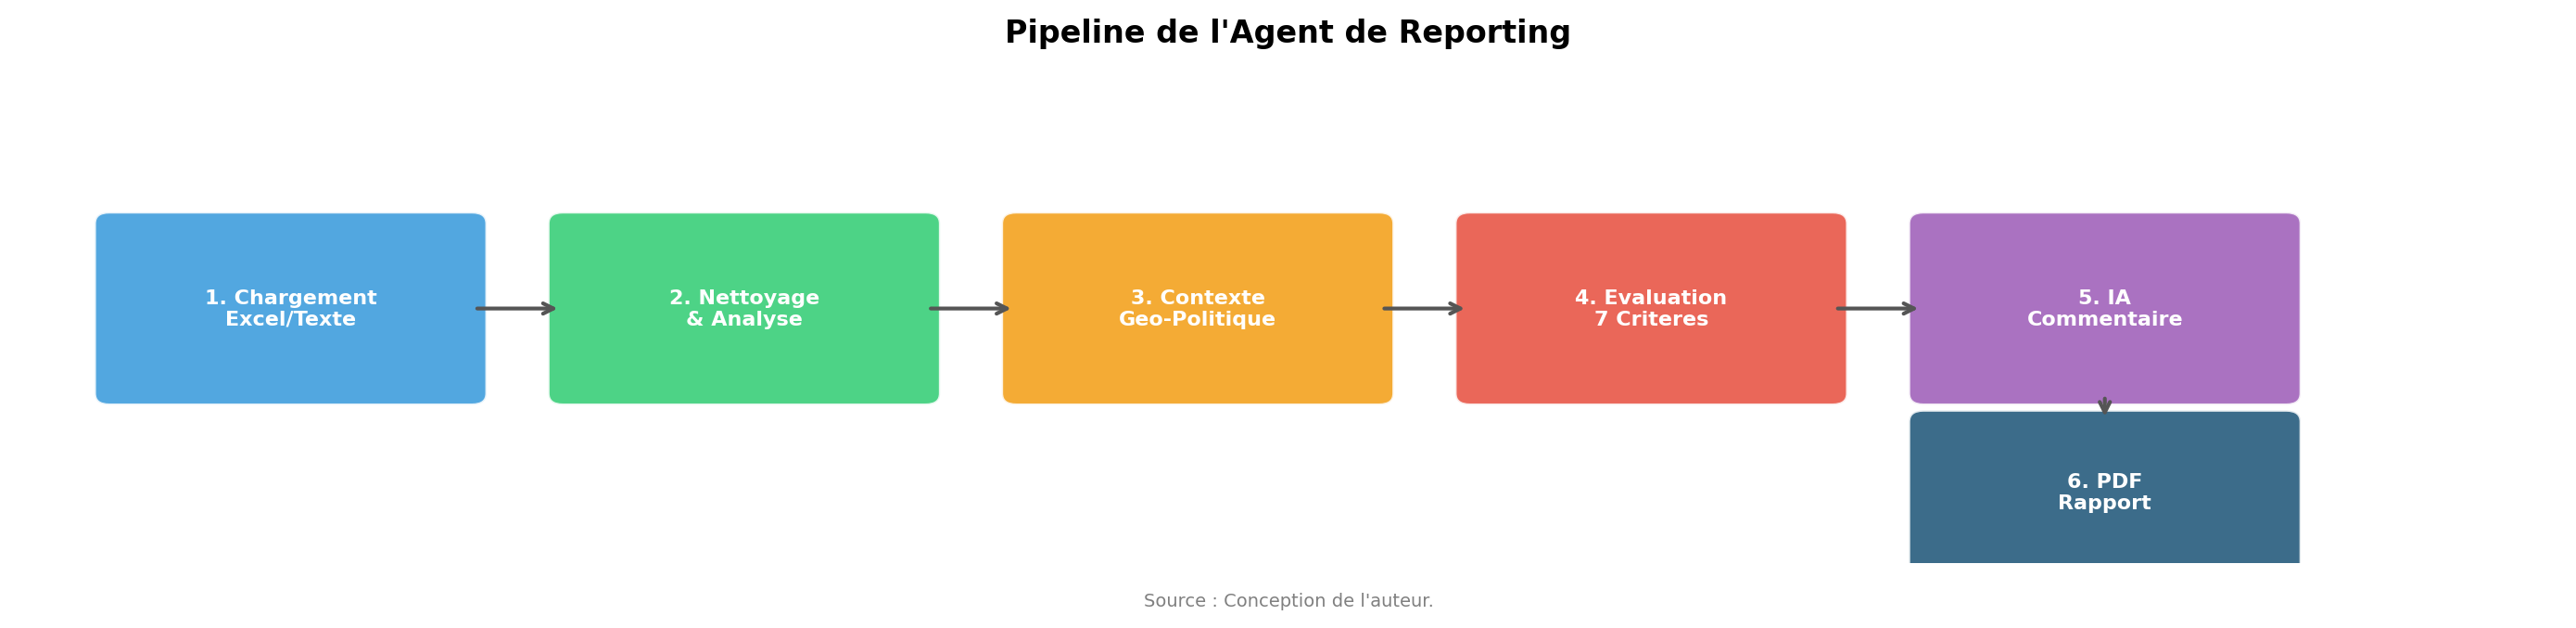
\includegraphics[width=0.95\textwidth]{pipeline_reporting.png}
\caption{Pipeline methodologique de l'agent de reporting, de l'ingestion au rapport PDF}
\label{fig:pipeline}
\textit{Source : Elaboration de l'auteur.}
\end{figure}

\section{Gestion de la dependance a l'API du modele de langage}

L'appel a l'API Groq pour la generation du commentaire narratif constitue une dependance externe non garantie (absence de cle API, quota depasse, latence reseau). Le module \texttt{ai\_agent.py} implemente un repli automatique (\textit{fallback}) : en l'absence de cle \texttt{GROQ\_API\_KEY} valide ou en cas d'exception lors de l'appel, l'agent genere un commentaire par gabarit textuel qui reprend les points forts et les points faibles identifies par le scoring, sans recourir au LLM. Cette conception garantit que le rapport PDF est toujours genere integralement, meme lorsque le service d'IA generative est indisponible -- un critere de robustesse essentiel pour un outil destine a un usage operationnel repete.

\textbf{Synthese du chapitre.} La methodologie decrite combine un pipeline de nettoyage tolerant aux donnees heterogenes, une base de connaissances contextuelle codee en dur, un moteur de scoring pondere et justifie critere par critere, une strategie de clarification conversationnelle, un mecanisme de protection des donnees personnelles aligne sur les pratiques existantes du PADESCE, et une strategie de validation par cas d'usage reel plutot que par echantillon statistique. Le chapitre suivant applique cette methodologie au cas reel du prestataire AMIFO-CIG et presente les resultats obtenus.

\newpage

% =====================================================
% CHAPITRE 3
% =====================================================

\chapter{Contexte, implementation et resultats}

\section{Contexte du PADESCE et de NAUMUR}

Le PADESCE associe des acteurs institutionnels, des prestataires de formation et une unite de coordination du projet, avec un mecanisme de verification independante des resultats (WORLD BANK, 2020). NAUMUR intervient dans ce dispositif comme organisation de suivi telephonique et de reporting, chargee de collecter et de synthetiser les donnees produites par les prestataires afin d'informer les decisions d'investissement du PADESCE. L'agent de reporting concu dans ce memoire s'inscrit dans cette mission : il vise a industrialiser une tache aujourd'hui realisee manuellement par les charges de suivi de NAUMUR.

\section{Architecture technique et outils utilises}
\label{sec:outils}

L'agent est implemente en Python, sous forme d'un paquet \texttt{reporting\_agent} comportant six modules : \texttt{data\_analyzer.py} (ingestion et nettoyage Excel), \texttt{cameroon\_context.py} (base de connaissances), \texttt{evaluator.py} (scoring multicritere, questions de suivi, recommandations d'investissement), \texttt{ai\_agent.py} (commentaire narratif via Groq/Llama), \texttt{report\_generator.py} (graphiques et rapport PDF) et \texttt{main.py} (orchestration du pipeline). Le tableau~\ref{tab:outils} presente les principaux outils mobilises.

\begin{table}[H]
\centering
\caption{Outils et technologies utilises}
\label{tab:outils}
\begin{tabularx}{\textwidth}{>{\bfseries}l X}
\toprule
Outil & Utilisation \\
\midrule
Python 3.13 & Langage de programmation de l'ensemble du pipeline \\
pandas & Lecture, nettoyage et analyse des classeurs Excel de prestataires \\
openpyxl & Moteur de lecture des fichiers \texttt{.xlsx} utilise par pandas \\
NumPy & Calculs numeriques (moyennes de completude, agregations) \\
Matplotlib & Generation des graphiques integres au rapport (barres de score, jauge, diagramme genre, completude) \\
ReportLab (\textit{platypus}) & Composition du document PDF final (tableaux, paragraphes, images, mise en page brandee) \\
Groq API / Llama & Generation du commentaire narratif en langage naturel a partir du score deja calcule \\
Django & Framework web de l'application Call App, dans laquelle l'agent est destine a etre integre \\
Git & Gestion de version du code \\
\LaTeX & Composition du present memoire \\
\bottomrule
\end{tabularx}
\textit{Source : Elaboration de l'auteur.}
\end{table}

La figure~\ref{fig:logos_outils} presente les logos des principaux outils mobilises.

\begin{figure}[H]
\centering
\begin{tabular}{>{\centering\arraybackslash}p{3.5cm} >{\centering\arraybackslash}p{3.5cm} >{\centering\arraybackslash}p{3.5cm}}

\includegraphics[height=1.2cm]{logo_numpy.png} &

\includegraphics[height=1.2cm]{logo_django.png} &

\includegraphics[height=1.2cm]{logo_git.png} \\
\footnotesize NumPy & \footnotesize Django & \footnotesize Git \\
\end{tabular}
\caption{Logos de trois des principaux outils et bibliotheques utilises (pandas, Matplotlib, ReportLab et Groq completent la chaine technique, cf. tableau~\ref{tab:outils})}
\label{fig:logos_outils}
\textit{Source : Sites officiels des projets respectifs.}
\end{figure}

\section{Deroulement du cas reel AMIFO-CIG}

Pour verifier le fonctionnement de bout en bout de l'agent, un test a ete conduit sur un classeur Excel reel, \texttt{Liste\_Apprenants\_calendrier\_AMIFO.xlsx}, transmis par le prestataire AMIFO-CIG (\textit{Prominent Youth for Development and Mutual Assistance CIG}), actif dans les villes de Kumba et Tiko, region du Sud-Ouest -- une zone directement concernee par la crise anglophone documentee dans la base de connaissances (section~\ref{sec:criteres} du chapitre 2).

\subsection{Ingestion et analyse automatique}

L'agent a identifie automatiquement 28 apprenants, 9 formations distinctes (gestion de cooperatives, elevage porcin, apiculture, elevage d'escargots, amelioration de la productivite porcine par insemination artificielle, production avicole, production de mais simplifiee), 7 seances planifiees et 3 lieux de formation (les graphies « KUMBA » et « Kumba » ayant ete comptees separement, illustrant la limite de deduplication discutee au chapitre 2). La region Sud-Ouest a ete correctement inferee a partir des villes citees, sans que l'utilisateur n'ait besoin de la preciser.

Le score de completude des donnees calcule automatiquement est de 25,8\,\%, plusieurs colonnes du fichier source (arrondissement, ville de la formation, fenetre de collecte, intitules detailles de formation) etant tres partiellement renseignees, tandis que d'autres (numero de ligne, ville de residence, genre, fonction) le sont a plus de 60\,\%. Cette heterogeneite typique d'un fichier de terrain a directement declenche, dans la logique de l'agent, une alerte de completude et une question de suivi invitant a completer les donnees manquantes.

\subsection{Reponses aux questions de suivi}

Conformement a la strategie decrite au chapitre 2, l'agent a soumis des questions de clarification, auxquelles les reponses suivantes ont ete fournies pour ce test : un niveau de satisfaction declare de 4 sur 5, la mention d'incidents lies a des coupures reseau recurrentes pendant les seances, et des mesures d'adaptation au contexte local consistant en l'organisation de sessions mobiles et l'usage ponctuel de generateurs electriques pour pallier les coupures.

\subsection{Resultat de l'evaluation multicritere}

Le tableau~\ref{tab:criteres_amifo} presente le detail des huit criteres pour le prestataire AMIFO-CIG. Chaque ligne est justifiee individuellement dans le rapport genere (voir figure~\ref{fig:pdf_page4}, section~\ref{sec:justif_criteres}).

\begin{longtable}{>{\bfseries}p{4cm} c c l p{5cm}}
\caption{Evaluation multicritere du prestataire AMIFO-CIG}
\label{tab:criteres_amifo} \\
\toprule
Critere & Score & Poids & Niveau & Detail \\
\midrule
\endfirsthead
\toprule
Critere & Score & Poids & Niveau & Detail \\
\midrule
\endhead
Completude des donnees & 36\,\% & 15\,\% & Insuffisant & Score de completude Excel : 25,8\,\% \\
Volume d'apprenants & 93\,\% & 12\,\% & Fort & 28 apprenants detectes \\
Diversite des formations & 100\,\% & 12\,\% & Fort & 9 formations identifiees \\
Pertinence sectorielle & 22\,\% & 13\,\% & Insuffisant & 2 formations sur 9 alignees avec les vocations economiques locales (elevage, agriculture) \\
Parite de genre & 82\,\% & 10\,\% & Fort & 41\,\% de femmes (11F / 16M) \\
Couverture geographique & 100\,\% & 10\,\% & Fort & 3 lieux de formation : Kumba, Kumba, Tiko \\
Adaptation au contexte local & 75\,\% & 15\,\% & Fort & Zones a difficulte moyenne de 50\,\% ; defis identifies : crise anglophone, insecurite, coupures reseau \\
Qualite de la planification & 100\,\% & 15\,\% & Fort & 7 seances planifiees \\
\midrule
\textbf{Score global} & \textbf{75,9\,\%} & \textbf{100\,\%} & \textbf{Excellent} & -- \\
\bottomrule
\end{longtable}

Le score global de 75,9\,\% place AMIFO-CIG dans la categorie \hyperref[sec:justif_criteres]{Excellent}, malgre une completude de donnees et une pertinence sectorielle jugees insuffisantes : le volume d'apprenants, la diversite des formations, la couverture geographique, la parite de genre et l'adaptation au contexte local compensent largement ces deux points faibles dans la somme ponderee. Ce resultat illustre concretement l'interet d'un score decompose critere par critere plutot que d'un jugement global unique : un gestionnaire PADESCE peut immediatement identifier que l'effort a fournir en priorite porte sur la qualite du reporting Excel et sur l'alignement des formations proposees avec les vocations economiques locales (elevage, agriculture, artisanat), et non sur le volume d'activite du prestataire, deja satisfaisant.

\subsection{Justification detaillee par critere}
\label{sec:justif_criteres}

Le critere de completude des donnees (36\,\%, insuffisant) reflete directement le score de 25,8\,\% calcule sur le classeur source ; il ne remet pas en cause la qualite de la formation dispensee, mais signale un risque pour le suivi futur si la qualite du reporting ne s'ameliore pas. Le critere de pertinence sectorielle (22\,\%, insuffisant) indique que seules 2 des 9 formations dispensees (l'elevage porcin et l'apiculture) correspondent aux vocations economiques recommandees pour la region Sud-Ouest par la base de connaissances (aviculture, elevage porcin, agriculture, gestion de cooperatives, apiculture) ; les formations de gestion de cooperatives et de production avicole, pourtant recommandees, n'ont pas ete detectees comme parfaitement alignees en raison de variations de formulation dans les intitules du classeur source, ce qui suggere une marge d'amelioration du module de correspondance textuelle plutot qu'une reelle inadequation sectorielle.

Les six autres criteres atteignent le niveau « fort ». L'adaptation au contexte local (75\,\%) valorise le fait que le prestataire opere dans une zone a difficulte moyenne (crise anglophone, coupures reseau) tout en ayant declare des mesures d'adaptation concretes (sessions mobiles, generateurs) lors des questions de suivi.

\section{Generation du rapport PDF et resultats visuels}

Le pipeline complet -- ingestion, enrichissement contextuel, scoring, generation des graphiques, commentaire IA et mise en page -- a produit un rapport PDF de six pages, \texttt{rapport\_AMIFO-CIG\_20260826\_093808.pdf}, consultable via le lien suivant :

\begin{center}
\href{run:../exports/rapport_AMIFO-CIG_20260826_093808.pdf}{\textbf{Consulter le rapport PDF complet genere par l'agent}}
\end{center}

\textit{Note : ce lien utilise la convention \texttt{\textbackslash href\{run:...\}} de \texttt{hyperref}, qui demande a certains lecteurs PDF (dont Adobe Acrobat et SumatraPDF) d'ouvrir un fichier local relatif au document courant. Son comportement depend du lecteur PDF utilise et des parametres de securite locaux ; certains lecteurs (dont plusieurs visualiseurs integres a un navigateur) l'ignorent silencieusement. Le fichier reste dans tous les cas disponible au chemin \texttt{exports/} du depot du projet.}

Les figures~\ref{fig:pdf_page1} a~\ref{fig:pdf_page6} presentent les six pages du rapport tel que reellement genere par l'agent sur ce cas.

\begin{figure}[H]
\centering
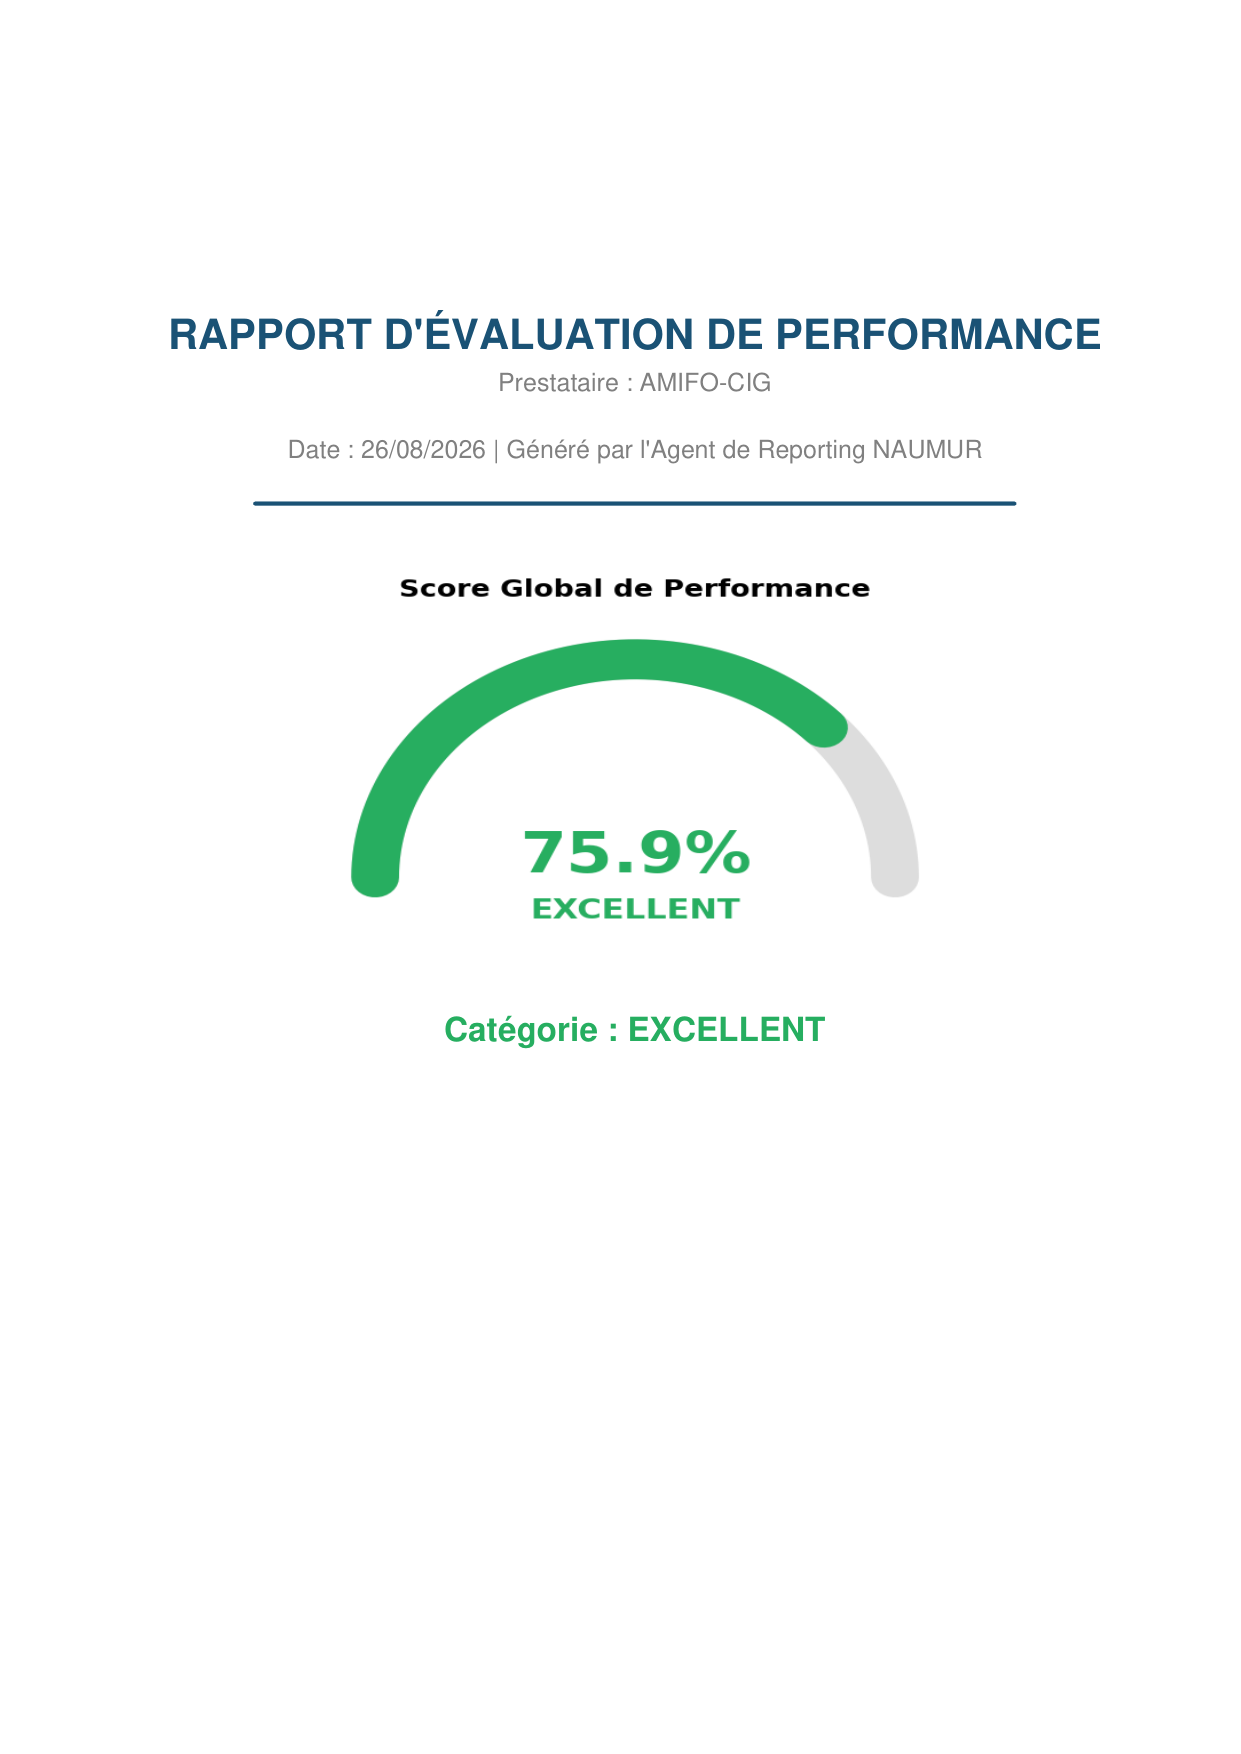
\includegraphics[width=0.85\textwidth]{reporting_agent_pdf_page1.png}
\caption{Rapport genere -- page 1 : page de couverture (logo NAUMUR, score global sous forme de jauge, categorie Excellent)}
\label{fig:pdf_page1}
\textit{Source : Capture d'ecran du rapport PDF genere par l'agent (cas AMIFO-CIG).}
\end{figure}

\begin{figure}[H]
\centering
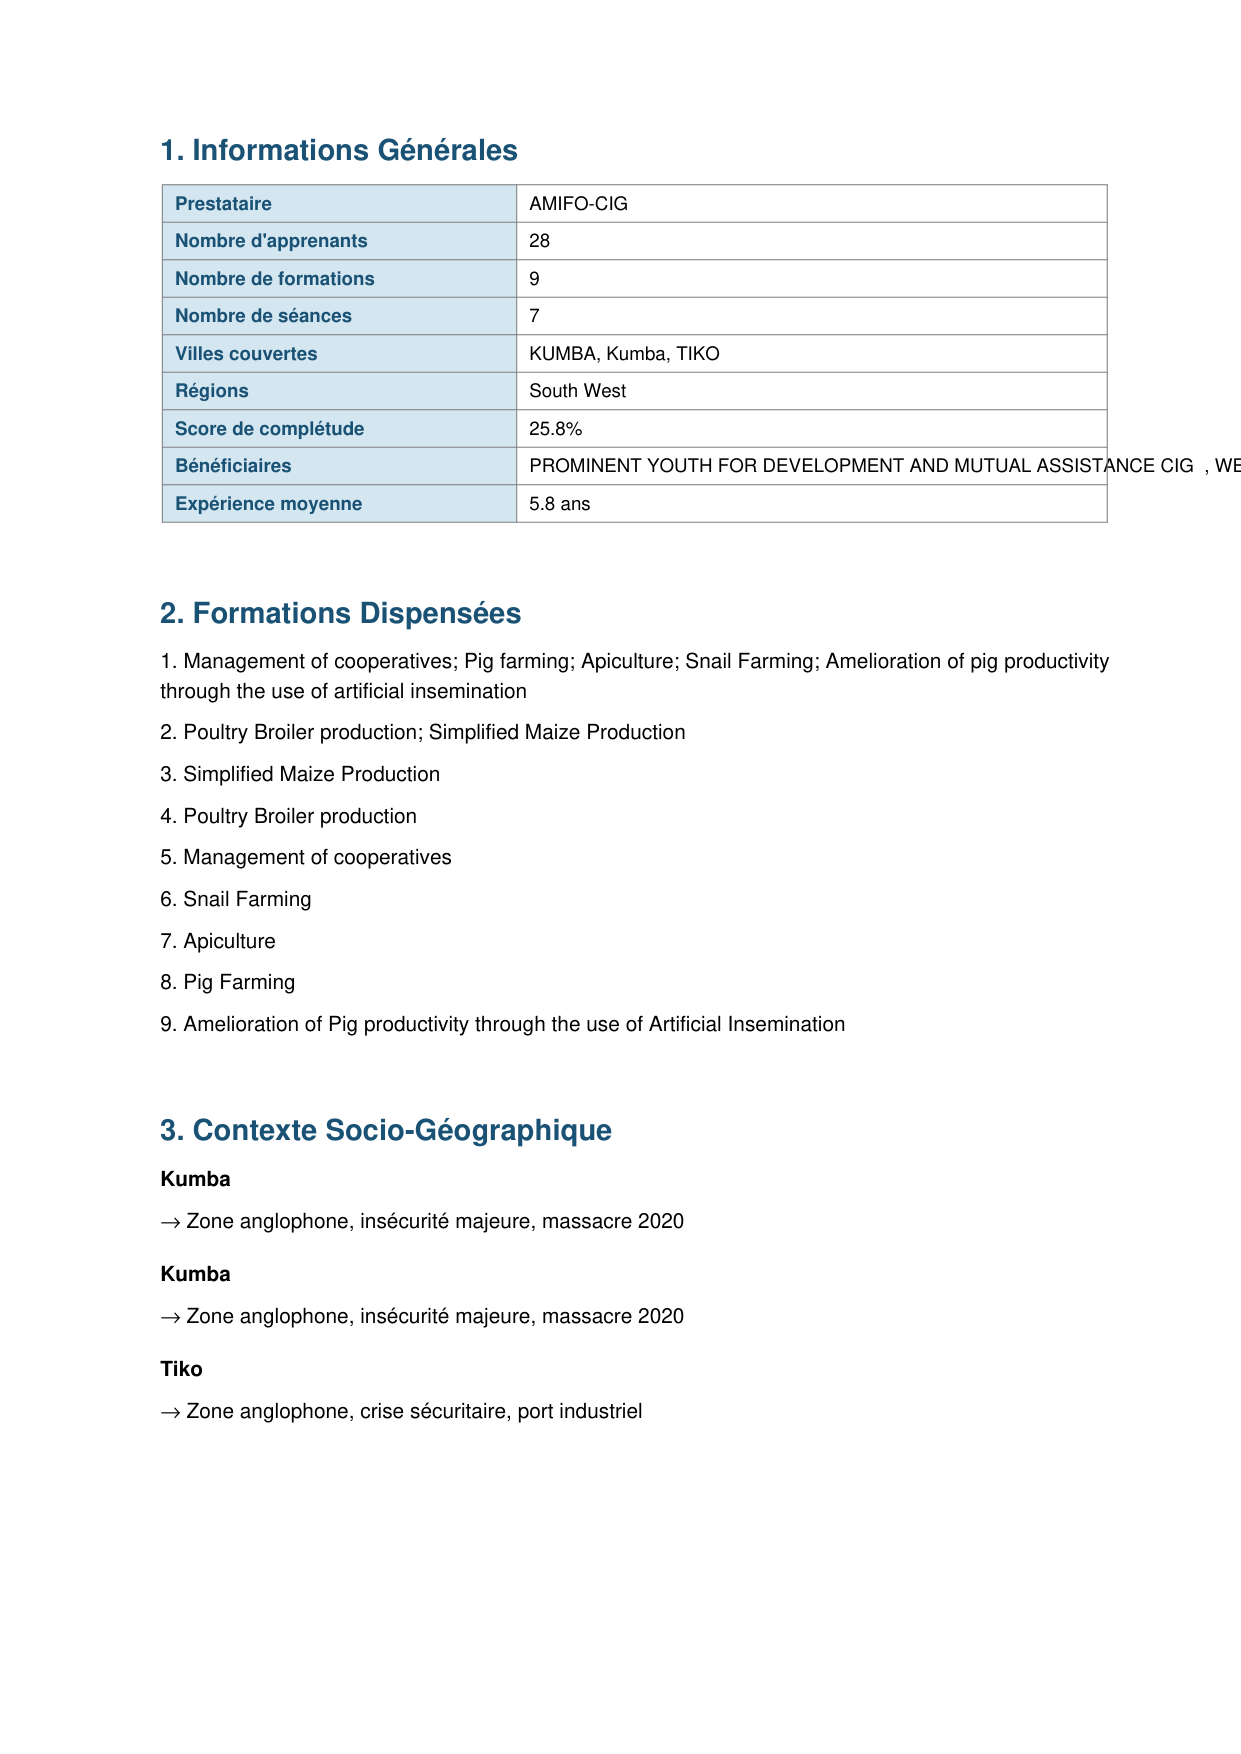
\includegraphics[width=0.85\textwidth]{reporting_agent_pdf_page2.png}
\caption{Rapport genere -- page 2 : informations generales, formations dispensees et contexte socio-geographique enrichi automatiquement}
\label{fig:pdf_page2}
\textit{Source : Capture d'ecran du rapport PDF genere par l'agent (cas AMIFO-CIG).}
\end{figure}

\begin{figure}[H]
\centering
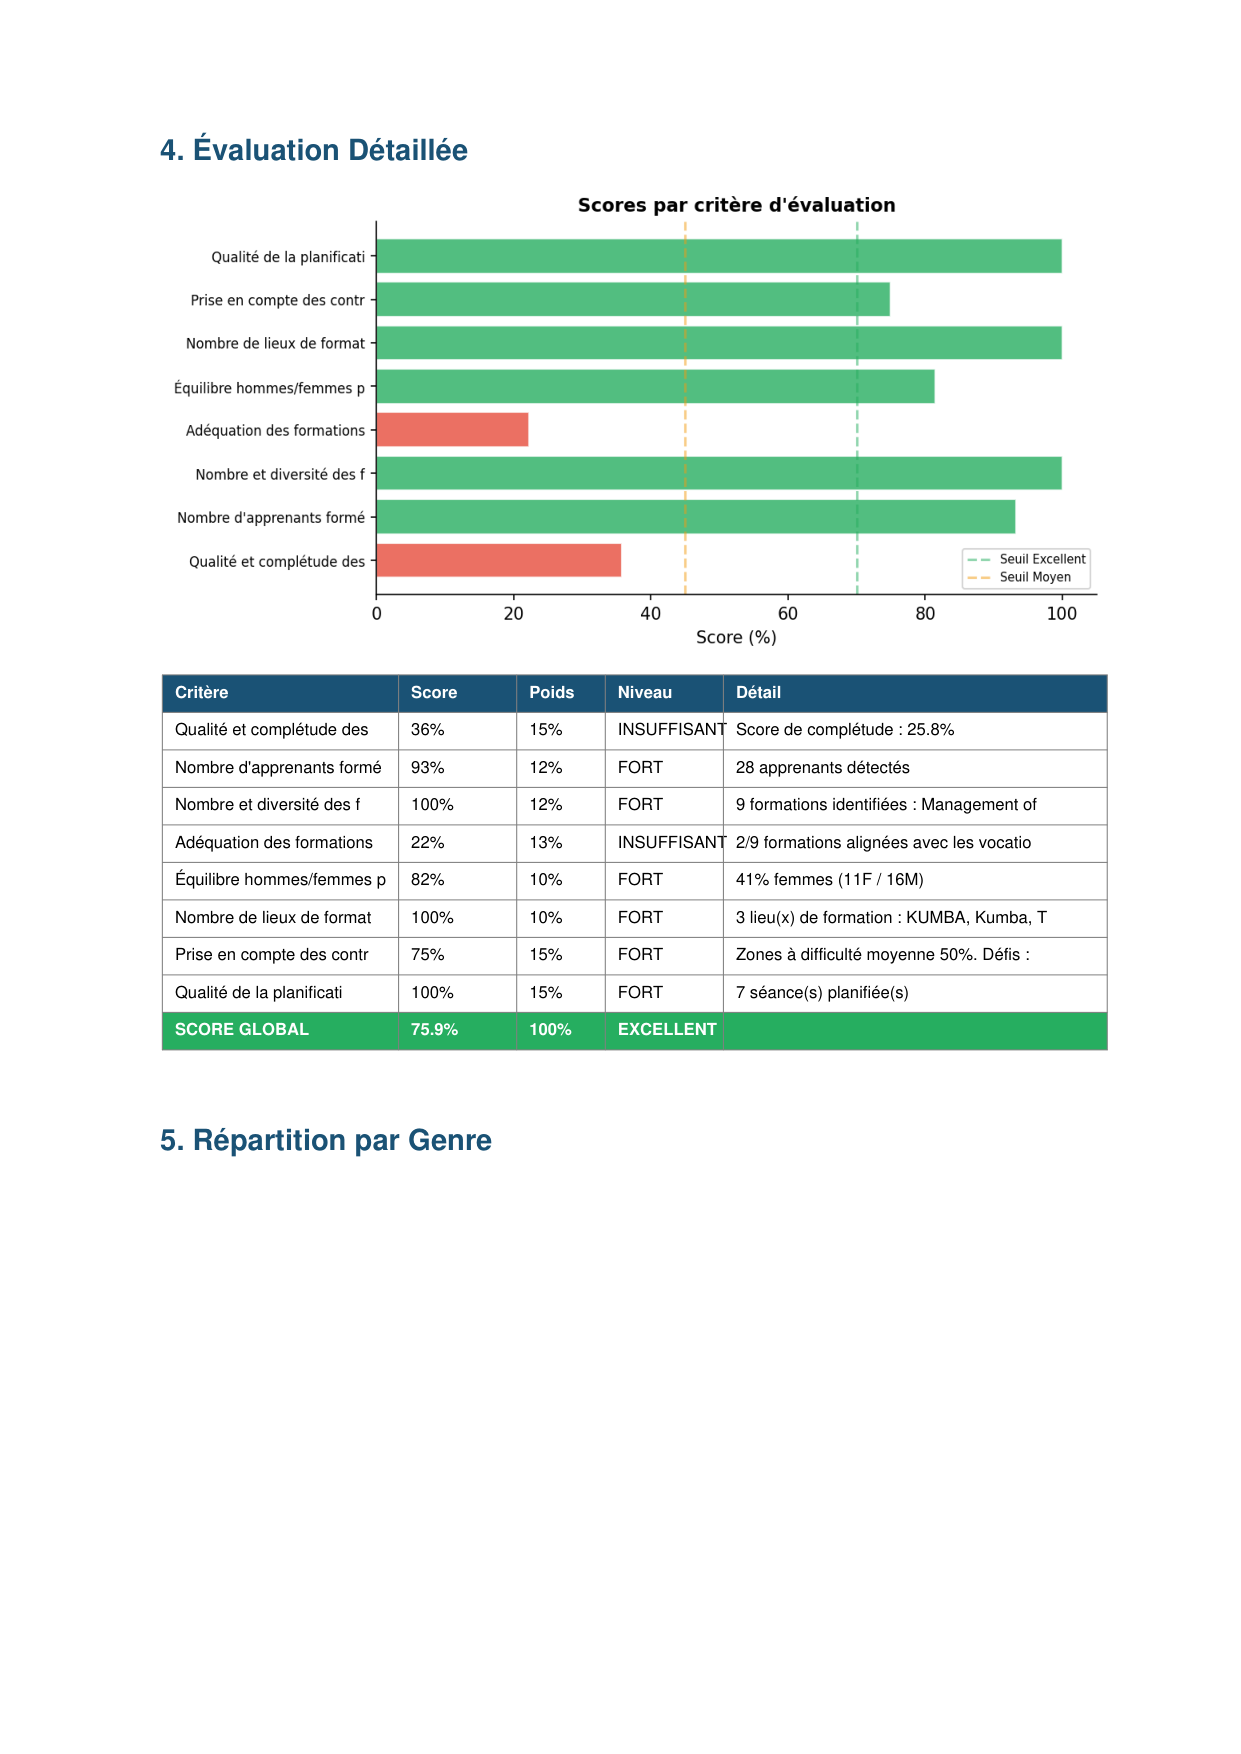
\includegraphics[width=0.85\textwidth]{reporting_agent_pdf_page3.png}
\caption{Rapport genere -- page 3 : evaluation detaillee, graphique des scores par critere et tableau recapitulatif}
\label{fig:pdf_page3}
\textit{Source : Capture d'ecran du rapport PDF genere par l'agent (cas AMIFO-CIG).}
\end{figure}

\begin{figure}[H]
\centering
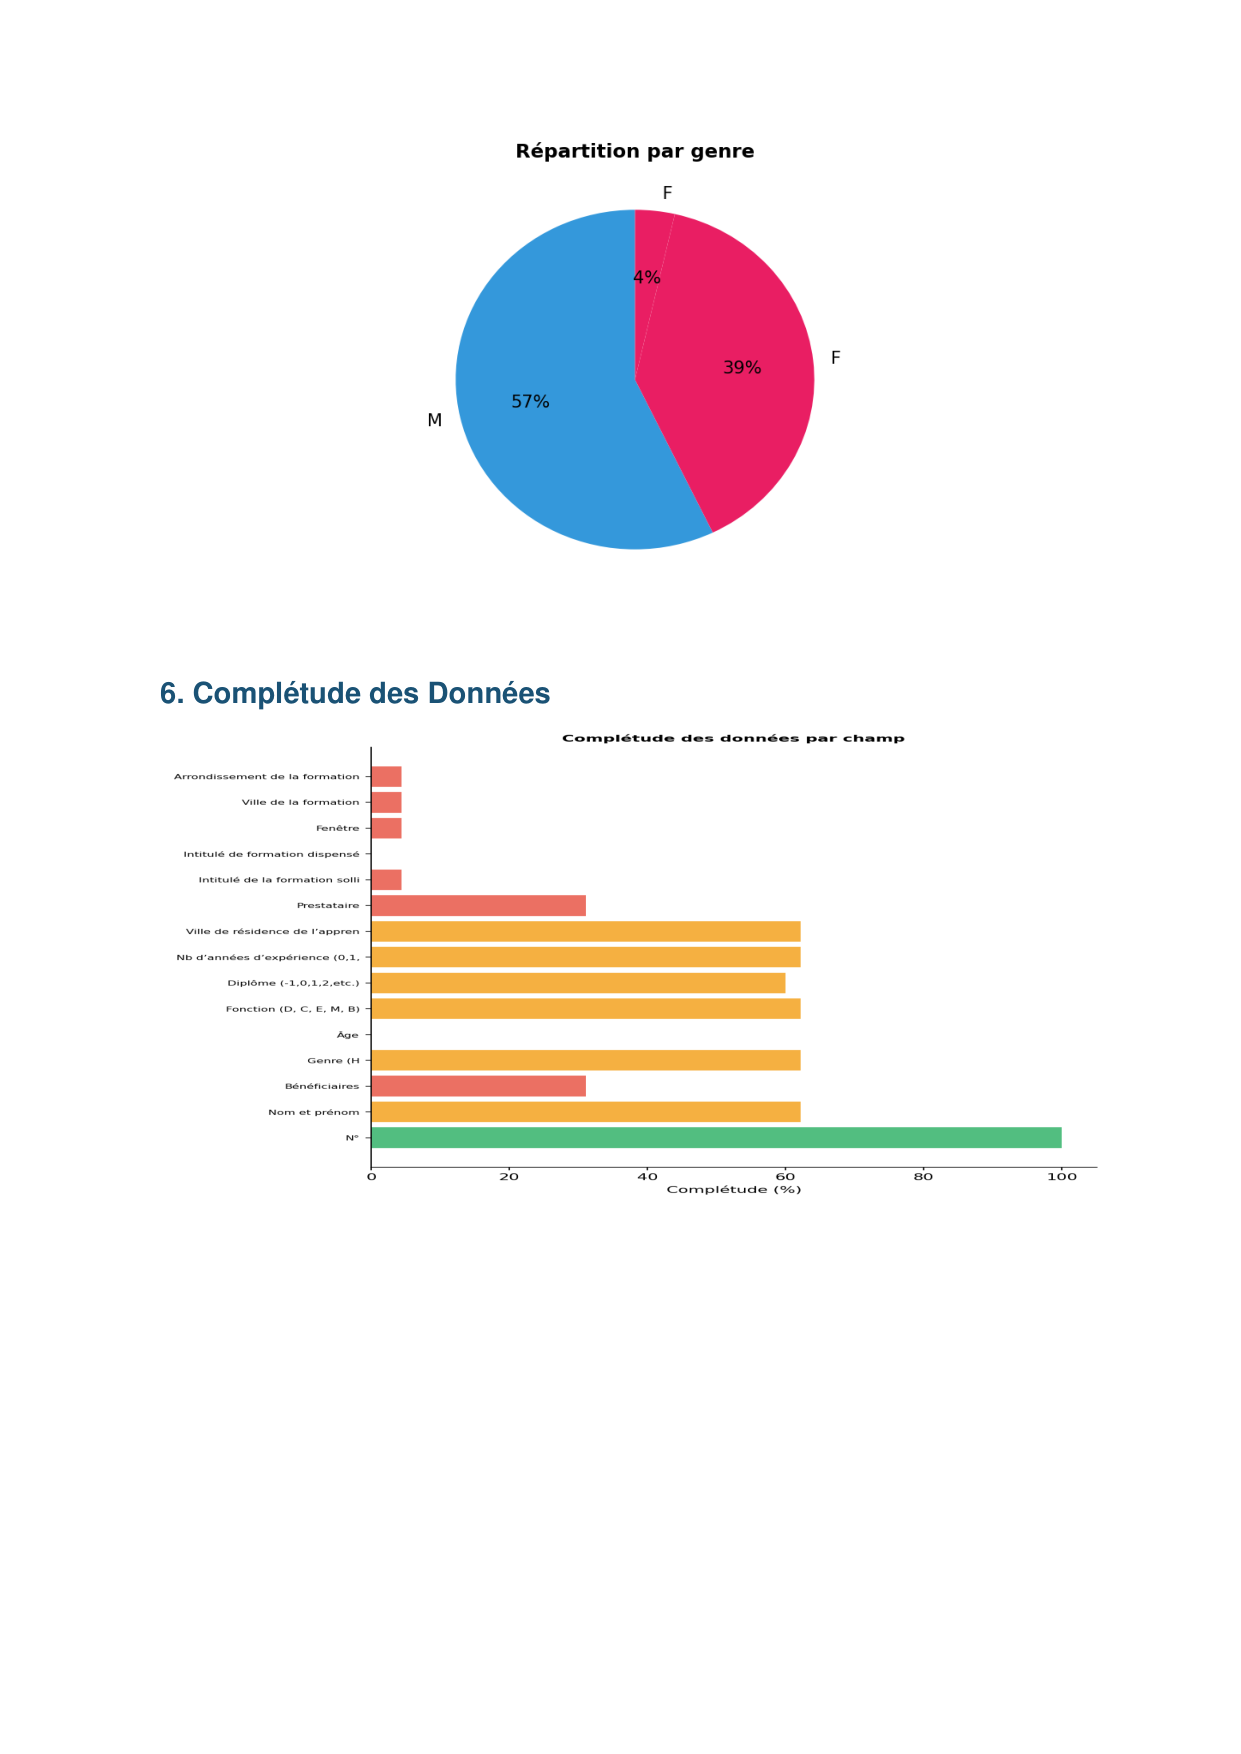
\includegraphics[width=0.85\textwidth]{reporting_agent_pdf_page4.png}
\caption{Rapport genere -- page 4 : repartition par genre et completude des donnees par champ (diagnostic visuel des colonnes lacunaires)}
\label{fig:pdf_page4}
\textit{Source : Capture d'ecran du rapport PDF genere par l'agent (cas AMIFO-CIG).}
\end{figure}

\begin{figure}[H]
\centering
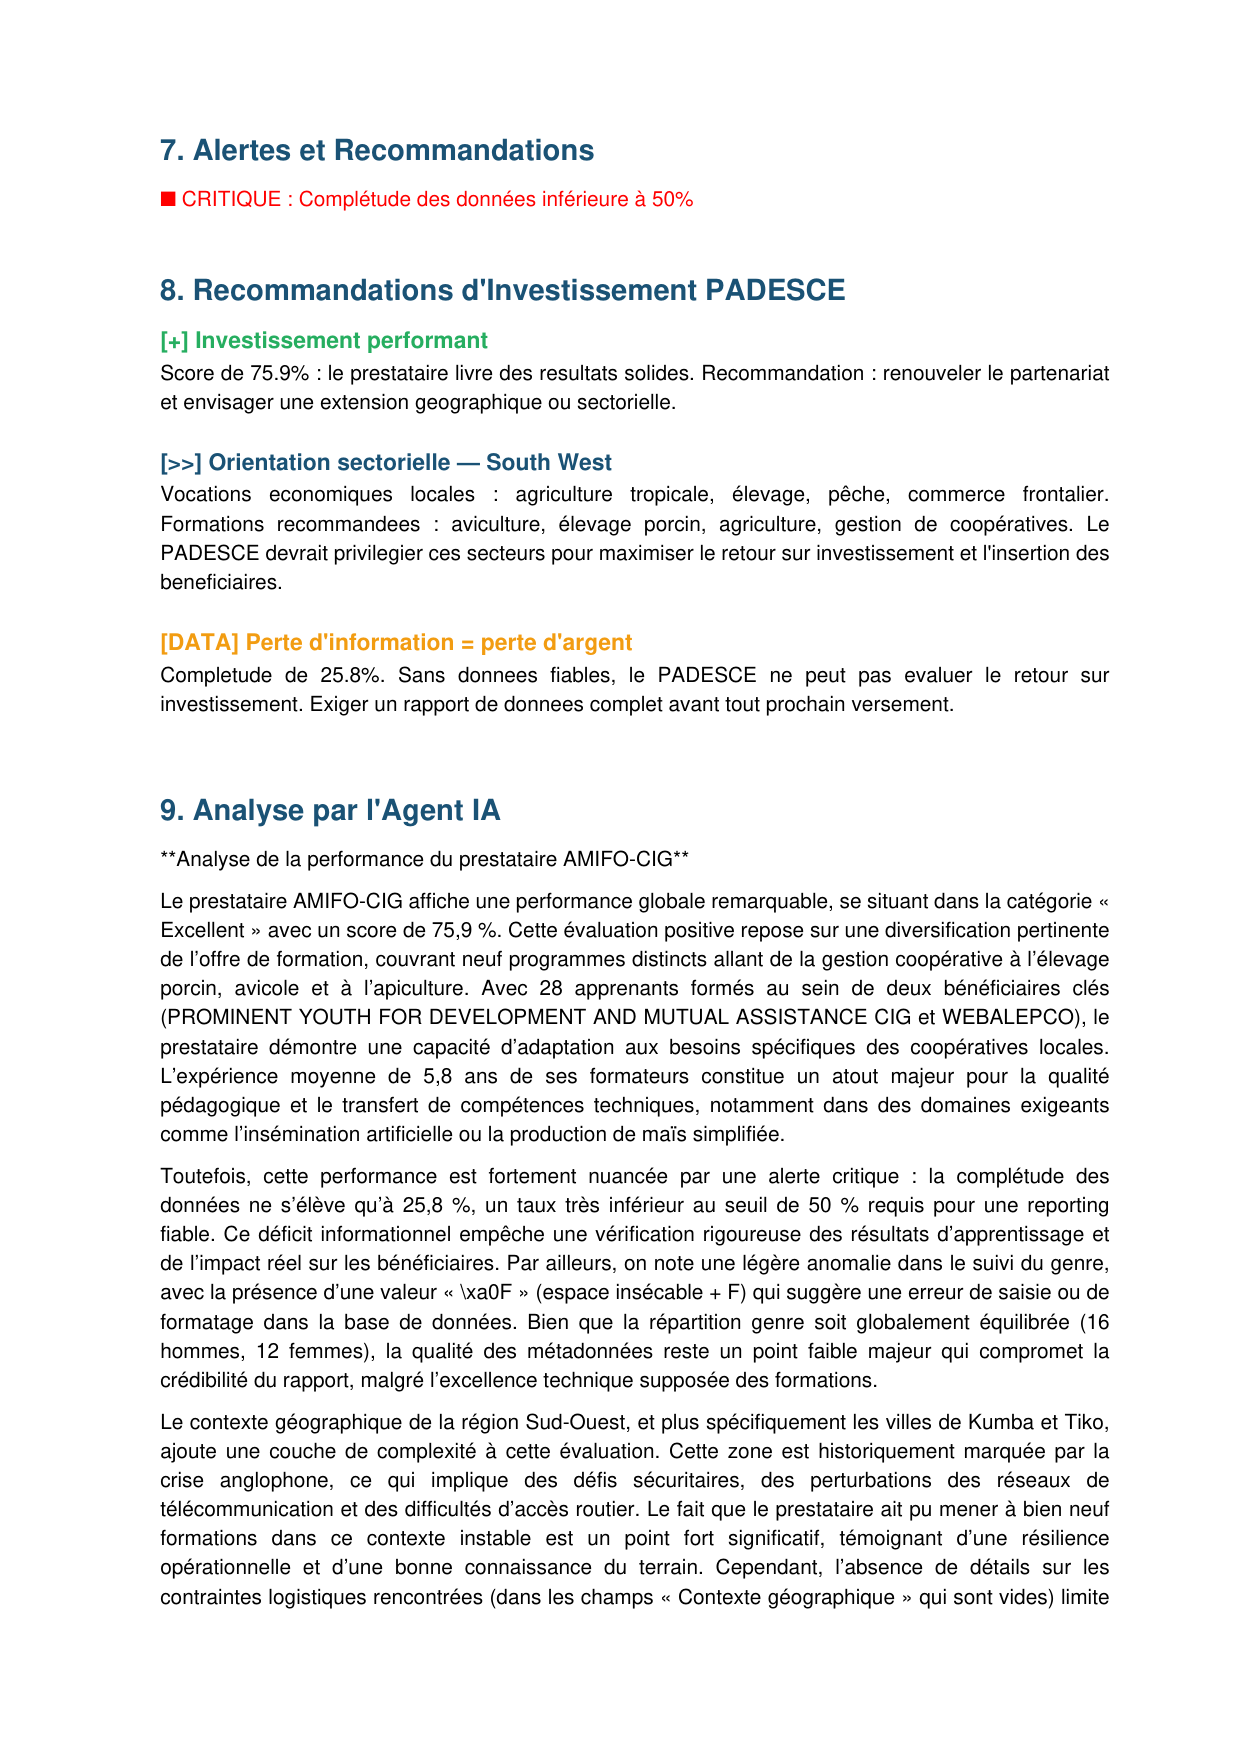
\includegraphics[width=0.85\textwidth]{reporting_agent_pdf_page5.png}
\caption{Rapport genere -- page 5 : alertes et recommandations d'investissement pour le PADESCE (zones a risque, orientation sectorielle)}
\label{fig:pdf_page5}
\textit{Source : Capture d'ecran du rapport PDF genere par l'agent (cas AMIFO-CIG).}
\end{figure}

\begin{figure}[H]
\centering
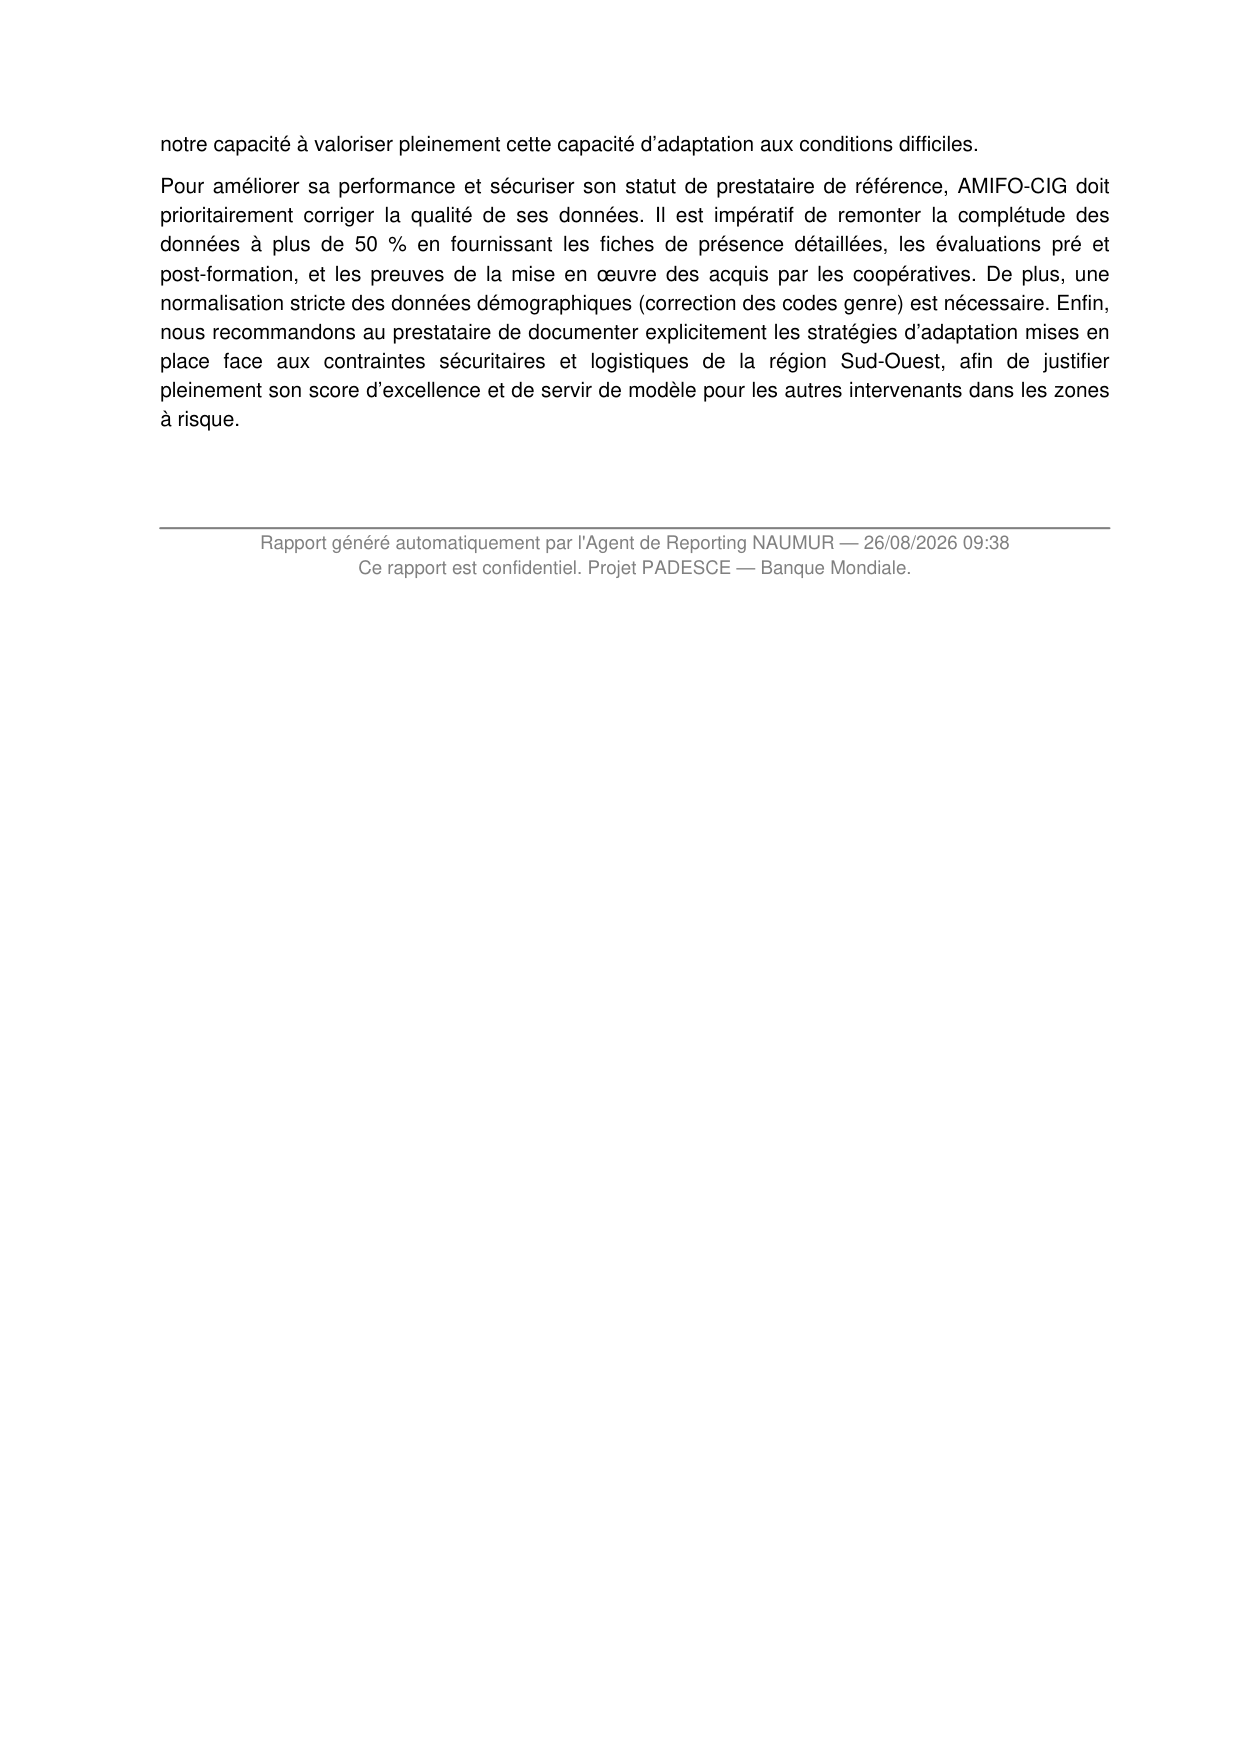
\includegraphics[width=0.85\textwidth]{reporting_agent_pdf_page6.png}
\caption{Rapport genere -- page 6 : commentaire narratif produit par le LLM (Llama via Groq) et pied de page de confidentialite}
\label{fig:pdf_page6}
\textit{Source : Capture d'ecran du rapport PDF genere par l'agent (cas AMIFO-CIG).}
\end{figure}

\section{Analyse critique du resultat obtenu}

Le resultat obtenu (Excellent, 75,9\,\%) doit etre lu avec la meme prudence que le systeme reclame pour lui-meme : il resulte de regles de ponderation choisies par conception, non d'un ajustement statistique optimal, et repose sur un unique cas reel traite jusqu'ici. La coherence interne du resultat est neanmoins verifiable point par point : chaque score de critere est retrace jusqu'a une donnee source ou une reponse de suivi identifiable, ce qui permet un audit complet -- une propriete qu'un modele d'apprentissage automatique boite noire n'offrirait pas nativement.

Le cas AMIFO-CIG illustre egalement une limite operationnelle concrete : la detection de deux lieux distincts pour une meme ville (« KUMBA » et « Kumba ») a artificiellement gonfle le score de couverture geographique. Sans consequence sur la categorie finale ici (le score de couverture etait deja plafonne a 100\,\%), ce type d'artefact pourrait, dans un autre cas, faire basculer un prestataire d'une categorie a l'autre ; il constitue une priorite identifiee pour la prochaine iteration du module de nettoyage (chapitre 4).

\section{Deploiement et integration dans l'application Call App}

L'agent de reporting est concu pour etre integre a l'application Call App du PADESCE, deja utilisee par les equipes de NAUMUR pour le suivi telephonique des beneficiaires, selon les principes suivants :

\begin{enumerate}
\item un charge de suivi televerse le classeur Excel d'un prestataire (ou saisit une description en texte libre) directement depuis l'interface Call App ;
\item l'agent execute le pipeline complet (nettoyage, enrichissement, scoring, questions de suivi le cas echeant) et affiche le score et la categorie dans l'interface avant generation du PDF ;
\item le rapport PDF genere est telechargeable depuis Call App et archive avec un horodatage, le score obtenu et la version de la base de connaissances utilisee ;
\item toute mise a jour de la base de connaissances Cameroun ou des ponderations de criteres est versionnee et documentee, de sorte que deux rapports generes a des dates differentes restent comparables ou que leur ecart soit explicable.
\end{enumerate}

Cette integration prolonge l'usage deja fait de Call App pour la collecte de donnees d'appel et de suivi. La figure~\ref{fig:callapp_dashboard_live} montre le tableau de bord operationnel actuel de Call App (module Call Center NAUMUR), point d'entree depuis lequel un charge de suivi accede aux appels PADESCE, aux prestataires en demarrage et au module de rapport ; la figure~\ref{fig:callapp_reporting} montre la page de reporting existante (« Rapport de l'application »), destinee a accueillir la couche d'evaluation automatisee des prestataires decrite dans ce memoire.

\begin{figure}[H]
\centering
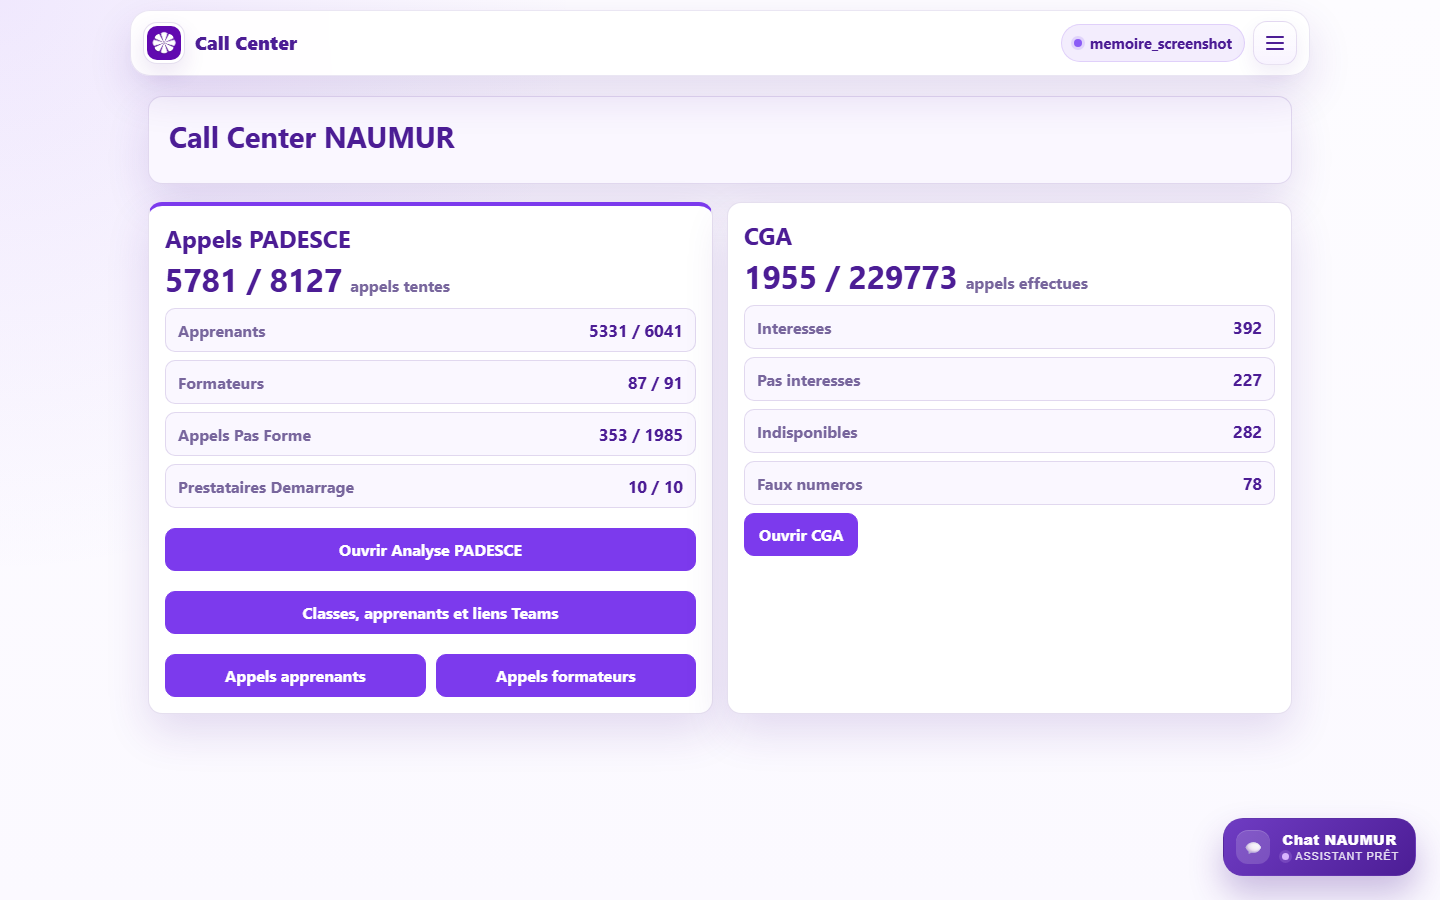
\includegraphics[width=0.85\textwidth]{callapp_dashboard_live.png}
\caption{Tableau de bord Call App -- vue d'ensemble des appels PADESCE et CGA en production}
\label{fig:callapp_dashboard_live}
\textit{Source : Capture d'ecran de l'application Call App (environnement de developpement, donnees reelles).}
\end{figure}

\begin{figure}[H]
\centering
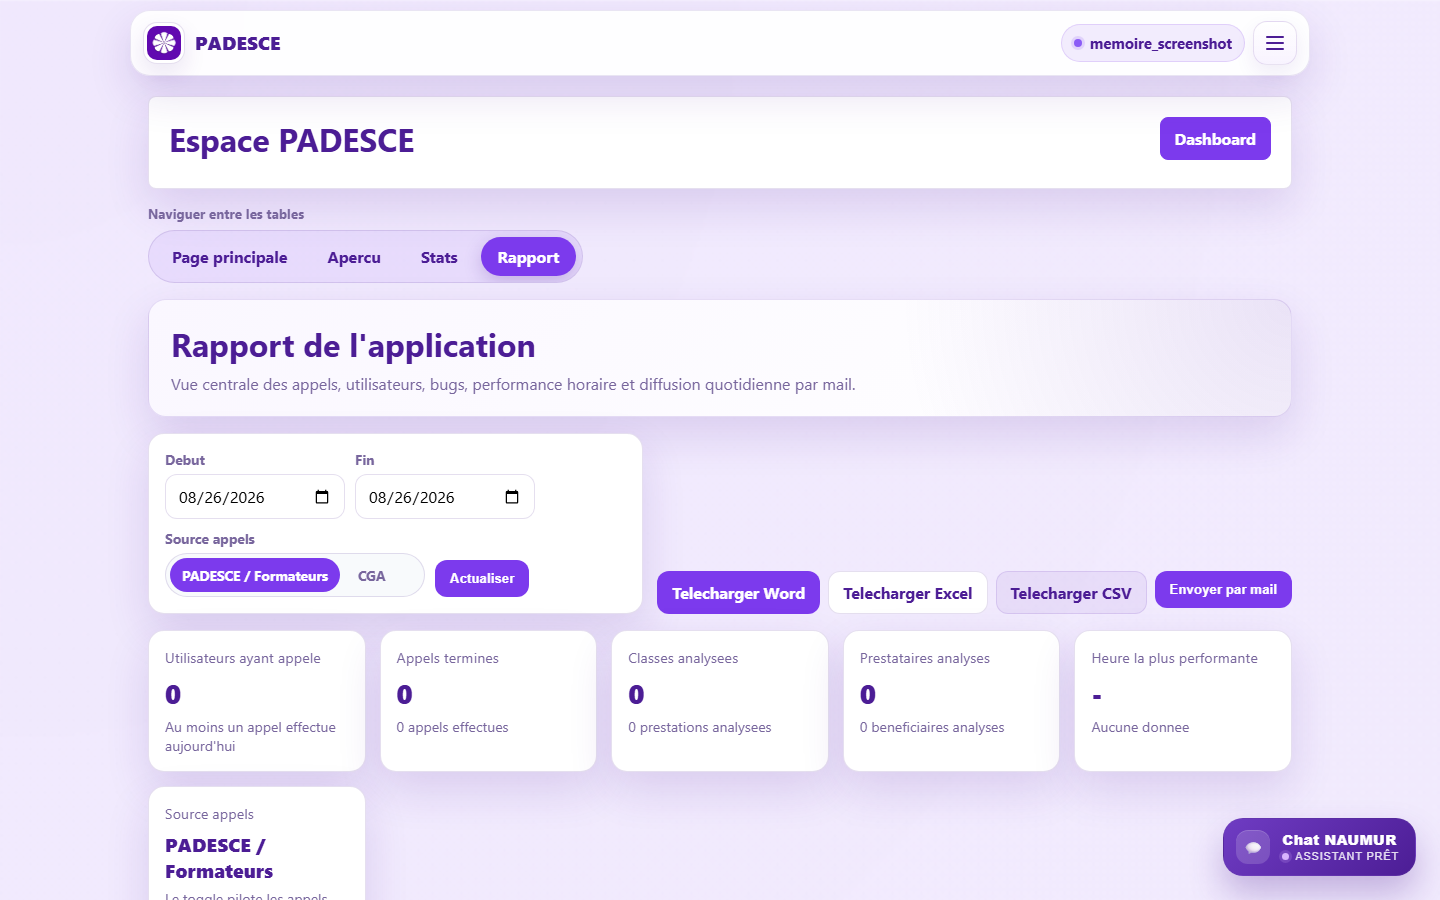
\includegraphics[width=0.85\textwidth]{callapp_rapport_prestations.png}
\caption{Page « Rapport de l'application » de Call App, module de reporting existant destine a integrer l'agent}
\label{fig:callapp_reporting}
\textit{Source : Capture d'ecran de l'application Call App (environnement de developpement).}
\end{figure}

\textbf{Synthese du chapitre.} L'application du pipeline au cas reel AMIFO-CIG demontre que l'agent produit, en quelques secondes, une evaluation multicritere justifiee, un jeu de recommandations d'investissement et un rapport PDF complet, a partir d'un classeur Excel non standardise. Le score de 75,9\,\% (categorie Excellent) est correctement decompose et audite critere par critere, et deux limites concretes ont ete identifiees : la deduplication insuffisante des noms de villes et la correspondance textuelle imparfaite entre intitules de formation et vocations recommandees. Le chapitre suivant discute ces limites plus generalement et propose une intervention pour la prochaine iteration.

\newpage

% =====================================================
% CHAPITRE 4
% =====================================================

\chapter{Discussion, limites et proposition d'intervention}

\section{Lecture generale des resultats}

Le principal resultat de ce travail n'est pas un score unique, mais la demonstration qu'un pipeline hybride regles + IA generative peut transformer, en quelques secondes, un classeur Excel heterogene en une evaluation multicritere justifiee, un jeu d'alertes actionnables et un rapport PDF pret a etre transmis a un decideur. Le cas AMIFO-CIG confirme que l'enrichissement automatique par la base de connaissances Cameroun apporte une information que l'evaluateur humain aurait sinon reconstituee manuellement (la crise anglophone au Sud-Ouest, les vocations economiques locales), et que la decomposition critere par critere permet d'orienter precisement l'action corrective (ici, la qualite du reporting et l'alignement sectoriel des formations).

\section{Discussion des hypotheses}

\subsection{Hypothese H1 : interpretabilite versus modele statistique}

H1 est soutenue par la conception meme du systeme : chaque score critere est retracable jusqu'a une donnee source verifiable, ce qu'un modele d'apprentissage automatique entraine sur un historique restreint de prestataires n'aurait pas pu garantir avec la meme fiabilite, compte tenu du risque de surapprentissage deja documente pour de petits echantillons (CAWLEY \& TALBOT, 2010). Cette hypothese n'a toutefois pas ete testee de maniere comparative : aucun modele d'apprentissage automatique n'a ete entraine en parallele sur les memes donnees pour objectiver l'ecart de performance predictive, faute d'un historique suffisant. L'argument reste donc principalement qualitatif et de conception, non empirique.

\subsection{Hypothese H2 : valeur ajoutee de l'enrichissement contextuel}

H2 est soutenue par l'observation directe du cas AMIFO-CIG : sans la base de connaissances, l'agent n'aurait pas pu generer automatiquement l'alerte de zone a risque, ni la recommandation d'orientation sectorielle vers l'elevage et l'agriculture, ni valoriser l'adaptation du prestataire au contexte de crise anglophone dans le score. Cette hypothese n'a cependant ete testee que sur un seul prestataire et une seule region ; sa robustesse sur d'autres regions (notamment celles au score de difficulte faible, ou l'effet du bonus contextuel est different) reste a verifier.

\subsection{Hypothese H3 : le nettoyage des donnees comme facteur limitant}

H3 est soutenue par le cas reel traite : l'artefact de deduplication des villes (« KUMBA » / « Kumba ») et l'imperfection de la correspondance textuelle entre intitules de formation et vocations recommandees ont eu davantage d'impact sur la justesse du score que n'importe quel choix de ponderation. Ce constat confirme que l'effort de developpement le plus rentable pour la prochaine iteration porte sur le pretraitement des donnees, non sur la sophistication de l'algorithme de scoring.

\section{Comparaison avec les approches alternatives}

Trois alternatives de conception ont ete ecartees et meritent d'etre explicitement discutees. Un modele d'apprentissage automatique pur (a la maniere des travaux de prediction educative recenses au chapitre 1) aurait pu, en theorie, capter des relations non lineaires entre variables, mais aurait exige un historique de prestataires bien plus large que celui disponible, et aurait ete plus difficile a auditer critere par critere -- un desavantage decisif pour un usage destine a justifier des decisions d'investissement. Un agent conversationnel purement generatif, sans moteur de regles ni base de connaissances codee, aurait ete plus rapide a prototyper, mais aurait expose le systeme a des hallucinations factuelles (par exemple sur la situation securitaire d'une region), un risque jugee inacceptable pour un usage institutionnel. L'architecture hybride retenue -- regles pour le score, base de connaissances codee pour les faits, LLM cantonne a la narration -- represente le compromis retenu entre rapidite de mise en \oe uvre, fiabilite factuelle et interpretabilite.

\section{Diagnostic des limites}

\subsection{Dependance a la qualite des donnees Excel sources}

Comme observe sur le cas AMIFO-CIG, la qualite du score reste directement dependante de la qualite du classeur source. Un prestataire produisant un fichier tres complet mais peu structure pourrait etre desavantage par des colonnes non reconnues par le detecteur de mots-cles, tandis qu'un prestataire produisant un fichier partiel mais bien nomme serait correctement traite. Cette dependance introduit un biais potentiel favorable aux prestataires les mieux equipes administrativement, independamment de la qualite reelle de la formation dispensee.

\subsection{Biais possible du commentaire genere par le LLM}

Le commentaire narratif genere par le modele de langage, bien que construit a partir d'un prompt contenant exclusivement les donnees et le score deja calcules, reste soumis aux biais generaux des grands modeles de langage (formulation trop generique, tonalite excessivement positive, reformulation imprecise d'un chiffre). Le score et la categorie affiches restent toutefois entierement determines par le moteur de regles, independamment du texte genere, ce qui limite l'impact d'un eventuel biais du LLM a la seule section narrative du rapport, clairement identifiee comme telle (page 6 du rapport, figure~\ref{fig:pdf_page6}).

\subsection{Base de connaissances Cameroun figee}

La base de connaissances regionale a ete constituee a un instant donne et necessite une mise a jour manuelle pour rester exacte -- une situation securitaire, une couverture reseau ou une vocation economique dominante peuvent evoluer sans que l'agent ne le detecte automatiquement. Ce choix, delibere pour garantir la stabilite et l'absence d'hallucination (chapitre 1), a pour contrepartie un risque d'obsolescence progressive si la maintenance n'est pas organisee.

\subsection{Absence de validation terrain multi-prestataires}

Le systeme n'a a ce stade ete valide que sur un seul prestataire reel (AMIFO-CIG). L'absence de test sur un ensemble plus large et plus divers de prestataires (autres regions, autres tailles, autres profils de completude de donnees) limite la portee des conclusions sur la robustesse generale du systeme de ponderation, notamment sur la pertinence des seuils de categorisation (45\,\% et 70\,\%) qui restent, a ce stade, un choix de conception non calibre empiriquement.

\section{Proposition d'intervention}

L'intervention proposee suit quatre axes prioritaires, resumes dans le tableau~\ref{tab:intervention}.

\begin{table}[H]
\centering
\caption{Plan d'intervention propose pour la prochaine iteration}
\label{tab:intervention}
\begin{tabularx}{\textwidth}{>{\bfseries}l X X}
\toprule
Axe & Action & Critere de passage \\
\midrule
1. Nettoyage & Normaliser les graphies de villes (correspondance approximative, table de synonymes) avant deduplication & Absence de doublons de ville sur un jeu de fichiers-test varie \\
2. Extension geographique & Etendre la base de connaissances a d'autres pays d'intervention du PADESCE ou de NAUMUR & Couverture validee par les equipes terrain \\
3. Entree en texte libre & Enrichir la comprehension du langage naturel (NLU) pour extraire automatiquement ville, formations et effectifs d'une description non structuree & Extraction correcte sur un corpus de descriptions reelles \\
4. Boucle de retour terrain & Recueillir systematiquement l'avis des evaluateurs PADESCE sur chaque score genere, pour recalibrer ponderations et seuils & Ecart mesure entre score de l'agent et jugement expert sur un echantillon multi-prestataires \\
\bottomrule
\end{tabularx}
\textit{Source : Elaboration de l'auteur.}
\end{table}

\subsection{Extension de la base de connaissances}

Au-dela du Cameroun, une extension de la base de connaissances a d'autres pays ou intervient NAUMUR permettrait de reutiliser directement l'architecture de l'agent, en respectant la meme structure de donnees (region, defis, vocations economiques, formations recommandees), sans modification du moteur de scoring.

\subsection{Entree texte libre plus riche}

L'entree en texte libre est aujourd'hui traitee de maniere minimale. Une extension via des techniques de comprehension du langage naturel permettrait d'extraire automatiquement d'une description telle que « On a un prestataire de la ville de Foumban, une trentaine d'apprenants en couture » les elements structures (ville, effectif, domaine de formation) necessaires au scoring, sans passer par un classeur Excel.

\subsection{Boucle de feedback des evaluateurs terrain}

La calibration actuelle des ponderations et des seuils de categorisation repose sur un jugement de conception, non sur un etalonnage empirique. Une boucle de feedback systematique -- ou chaque score genere est compare a l'avis d'un evaluateur PADESCE experimente -- permettrait d'ajuster progressivement les ponderations et de documenter les cas de desaccord, sans jamais recourir a un reentrainement statistique opaque.

\section{Conditions de reussite de la prochaine iteration}

La prochaine iteration pourra etre consideree comme concluante si quatre conditions sont reunies : une deduplication fiable des lieux et une correspondance textuelle robuste entre formations et vocations recommandees ; une extension testee de la base de connaissances a au moins un pays supplementaire ; une extraction fonctionnelle a partir de texte libre sur un corpus reel de descriptions de prestataires ; et un premier cycle de feedback documente avec les evaluateurs PADESCE sur un echantillon d'au moins une dizaine de prestataires couvrant plusieurs regions.

\textbf{Synthese du chapitre.} La discussion montre que les limites actuelles du systeme relevent principalement de la qualite du pretraitement des donnees et de l'etendue encore restreinte de la validation terrain, plutot que de la logique de scoring elle-meme. La reponse appropriee est une intervention ciblee sur le nettoyage, l'extension geographique de la base de connaissances, l'entree en texte libre et une boucle de feedback structuree avec les evaluateurs PADESCE, sans remettre en cause l'architecture hybride regles + IA generative retenue.

\newpage

% =====================================================
% CONCLUSION GENERALE
% =====================================================

\chapter*{Conclusion generale}
\addcontentsline{toc}{chapter}{Conclusion generale}

Ce memoire avait pour objectif de concevoir, implementer et tester un agent de reporting hybride pour l'evaluation de la performance des prestataires de formation du PADESCE, en combinant des regles metier explicites et une couche d'intelligence artificielle generative. Le travail a d'abord distingue l'agent de reporting d'un modele d'apprentissage automatique classique, en justifiant ce choix par l'absence d'un historique de donnees suffisant pour une generalisation statistique fiable et par l'exigence d'interpretabilite critere par critere posee par l'usage operationnel envisage.

Un agent complet a ete implemente sous forme de six modules Python : ingestion et nettoyage de classeurs Excel non standardises, base de connaissances socio-geo-demographique et politique des dix regions du Cameroun, moteur de scoring multicritere pondere sur huit dimensions, generateur de questions de clarification et de recommandations d'investissement, couche de generation narrative par un grand modele de langage (Llama, via Groq) avec repli automatique par gabarit, et generateur de rapport PDF brande NAUMUR combinant tableaux, graphiques et commentaire narratif.

Le systeme a ete valide sur un cas reel, le prestataire AMIFO-CIG, actif dans les villes de Kumba et Tiko en region du Sud-Ouest. L'agent a produit, en quelques secondes, un score global de 75,9\,\% et une categorie Excellent, en identifiant correctement deux points faibles (completude des donnees a 25,8\,\%, pertinence sectorielle de 22\,\%) largement compenses par un volume d'apprenants, une diversite de formations, une couverture geographique, une parite de genre et une adaptation au contexte local jugees fortes. Le rapport PDF genere de six pages, integrant graphiques, alertes et commentaire narratif, a ete verifie page par page et constitue une preuve de concept operationnelle directement exploitable.

La contribution du travail reside moins dans la sophistication algorithmique que dans la discipline de conception : separation stricte entre calcul deterministe du score et generation narrative par IA, base de connaissances codee en dur pour eviter toute hallucination factuelle sur des sujets sensibles (situation securitaire, contexte politique), justification systematique de chaque critere, et alignement du mecanisme de protection des donnees personnelles sur les pratiques deja en vigueur dans l'ecosysteme logiciel du PADESCE.

La suite prioritaire consiste a fiabiliser le nettoyage des noms de lieux et la correspondance entre formations et vocations economiques recommandees, a etendre la base de connaissances a d'autres pays d'intervention, a enrichir l'entree en texte libre par des techniques de comprehension du langage naturel, et a organiser une boucle de feedback structuree avec les evaluateurs terrain du PADESCE sur un echantillon plus large et plus divers de prestataires. Ces etapes conditionnent le passage d'une preuve de concept validee sur un cas unique a un outil de pilotage regulierement utilise par NAUMUR et le PADESCE.

\newpage

% =====================================================
% REFERENCES BIBLIOGRAPHIQUES
% =====================================================

\chapter*{References bibliographiques}
\addcontentsline{toc}{chapter}{References bibliographiques}

\begin{description}[leftmargin=0cm, itemsep=0.5em]

\item AL-SHABANDAR, R., HUSSAIN, A. J., LIATSIS, P., \& KEIGHT, R. (2019). Detecting At-Risk Students With Early Interventions Using Machine Learning Techniques. \textit{IEEE Access}, 7, 149464--149478.

\item ALSHAHRANI, A. (2025). SMOTE-Optimized Machine Learning Framework for Predicting Retention in Workforce Development Training. \textit{Computers, Materials \& Continua}, 85(2), 4067--4090.

\item BREIMAN, L. (2001). Random Forests. \textit{Machine Learning}, 45(1), 5--32.

\item CAWLEY, G. C., \& TALBOT, N. L. C. (2010). On Over-Fitting in Model Selection and Subsequent Selection Bias in Performance Evaluation. \textit{Journal of Machine Learning Research}, 11, 2079--2107.

\item DELONE, W. H., \& MCLEAN, E. R. (2003). The DeLone and McLean Model of Information Systems Success: A Ten-Year Update. \textit{Journal of Management Information Systems}, 19(4), 9--30.

\item DURDEVIC BABIC, I. (2015). Predicting Student Satisfaction with Courses Based on Log Data from a Virtual Learning Environment. \textit{Croatian Operational Research Review}, 6(1), 105--120.

\item GEBRU, T., MORGENSTERN, J., VECCHIONE, B., VAUGHAN, J. W., WALLACH, H., DAUME III, H., \& CRAWFORD, K. (2021). Datasheets for Datasets. \textit{Communications of the ACM}, 64(12), 86--92.

\item GITINABARD, N., KHOSHNEVISAN, F., LYNCH, C. F., \& WANG, E. Y. (2018). Your Actions or Your Associates? Predicting Certification and Dropout in MOOCs with Behavioral and Social Features. \textit{Proceedings of the 11th International Conference on Educational Data Mining}, 404--410.

\item KIRKPATRICK, D. L. (1996). Great Ideas Revisited: Revisiting Kirkpatrick's Four-Level Model. \textit{Training and Development}, 50(1), 54--59.

\item LUNDBERG, S. M., \& LEE, S.-I. (2017). A Unified Approach to Interpreting Model Predictions. \textit{Advances in Neural Information Processing Systems}, 30.

\item MITCHELL, M., WU, S., ZALDIVAR, A., BARNES, P., VASSERMAN, L., HUTCHINSON, B., SPITZER, E., RAJI, I. D., \& GEBRU, T. (2019). Model Cards for Model Reporting. \textit{Proceedings of the Conference on Fairness, Accountability, and Transparency}, 220--229.

\item OECD. (2019). \textit{Better Criteria for Better Evaluation: Revised Evaluation Criteria Definitions and Principles for Use (Guidance)}. OECD Publishing.

\item OECD. (2021). \textit{Applying Evaluation Criteria Thoughtfully (Guidance)}. OECD Publishing.

\item RIBEIRO, M. T., SINGH, S., \& GUESTRIN, C. (2016). ``Why Should I Trust You?'': Explaining the Predictions of Any Classifier. \textit{Proceedings of the 22nd ACM SIGKDD International Conference on Knowledge Discovery and Data Mining}, 1135--1144.

\item TABASSI, E. (2023). \textit{Artificial Intelligence Risk Management Framework (AI RMF 1.0)}. National Institute of Standards et Technology.

\item VARMA, S., \& SIMON, R. (2006). Bias in Error Estimation When Using Cross-Validation for Model Selection. \textit{BMC Bioinformatics}, 7(1), 91.

\item WORLD BANK. (2020). \textit{Secondary Education and Skills Development Project (P170561) -- Project Appraisal Document No PAD3439}. Washington, DC.

\item WORLD BANK. (2025a). \textit{Cameroun: Projet d'Appui au Developpement de l'Enseignement Secondaire et des Competences pour la Croissance et l'Emploi (PADESCE) -- Mission d'Assistance Technique du 17 au 21 novembre 2025 (Aide-memoire No 207783)}.

\item WORLD BANK. (2025b). \textit{Disclosable Restructuring Paper: Secondary Education and Skills Development Project (P170561) (Restructuring Paper No RES00864)}.

\item WORLD BANK. (2026). \textit{Disclosable Version of the ISR: Secondary Education and Skills Development Project (P170561), Sequence No. 10 (Implementation Status and Results Report No ISR06119)}.

\item ZENG, W., CHIN, S.-C., ZEIMET, B., KUANG, R., \& CHI, C.-L. (2017). Dropout Prediction in Home Care Training. \textit{Proceedings of the 10th International Conference on Educational Data Mining}, 442--447.

\end{description}

\newpage

% =====================================================
% TABLE DES MATIERES DETAILLEE
% =====================================================

\tableofcontents

\end{document}
